% Preamble del documento

\documentclass[11pt, a4paper, titlepage]{article}


%%%%%%%%%%%%%%%%%%%%%%%%%%%%%%%%%%%%%%%%%%%%%%%%%%%%%%%%%%%%%%%%%%%%%%%%%%%%%%%%%%%%%%%%%%%%%%%%
% Encoding e idioma Español,
%%%%%%%%%%%%%%%%%%%%%%%%%%%%%%%%%%%%%%%%%%%%%%%%%%%%%%%%%%%%%%%%%%%%%%%%%%%%%%%%%%%%%%%%%%%%%%%%
\usepackage[utf8]{inputenc}
\usepackage[spanish, es-tabla]{babel} % Para poner cuadro en vez de tabla, etc
%%%%%%%%%%%%%%%%%%%%%%%%%%%%%%%%%%%%%%%%%%%%%%%%%%%%%%%%%%%%%%%%%%%%%%%%%%%%%%%%%%%%%%%%%%%%%%%%



%%%%%%%%%%%%%%%%%%%%%%%%%%%%%%%%%%%%%%%%%%%%%%%%%%%%%%%%%%%%%%%%%%%%%%%%%%%%%%%%%%%%%%%%%%%%%%%%
% Paquetes
%%%%%%%%%%%%%%%%%%%%%%%%%%%%%%%%%%%%%%%%%%%%%%%%%%%%%%%%%%%%%%%%%%%%%%%%%%%%%%%%%%%%%%%%%%%%%%%%
\usepackage[colorlinks=true, urlcolor=cyan, citecolor=blue, linkcolor=blue, hidelinks]{hyperref} % /url{}, /ref{}...
\usepackage[a4paper,top=2cm,bottom=2cm,left=3cm,right=3cm,marginparwidth=1.75cm]{geometry}
\usepackage{minted} % Código
\usepackage{setspace}
\usepackage{pdfpages}

\usepackage[sorting=none, style=numeric]{biblatex} % aparece 1ro la 1ra citada
\addbibresource{citas.bib}

\usepackage[smartEllipses]{markdown}

\usepackage{amsmath}

\usepackage[utf8]{inputenc}

\usepackage[table]{xcolor} % Colores en tablas/texto/etc

\usepackage{graphicx} % Imágenes

\usepackage{tabularx} % Tablas más potentes
\usepackage{longtable} % Tablas muy largas
\usepackage{multirow}
\usepackage{booktabs}
\usepackage{multicol}
\usepackage{adjustbox} % Ajustar tablas al ancho de la página
\usepackage{pdflscape}

\usepackage{datetime} % Fechas
\usepackage{svg} % para el svg del logo de la eina
\usepackage{titlesec}
\usepackage[section]{placeins}  % para floatbarrier en secciones,
                                % con [section] se ponen silenciosamente en cada seccion

\usepackage{listliketab}
\usepackage{fancyhdr} %pagestyles adicionales

\usepackage{lmodern} % Fuente moderna, \code con negrita
\usepackage{caption} % para poner labels en tabular sin convertirlos en tablas que flotan

\makeatletter
%%%%%%%%%%%%%%%%%%%%%%%%%%%%%%%%%%%%%%%%%%%%%%%%%%%%%%%%%%%%%%%%%%%%%%%%%%%%%%%%%%%%%%%%%%%%%%%%
\renewcommand\paragraph{\@startsection{paragraph}{4}{\z@}%
            {-2.5ex\@plus -1ex \@minus -.25ex}%
            {1.25ex \@plus .25ex}%
            {\normalfont\normalsize\bfseries}} % no sé de donde ha salido esto
\makeatother
\setcounter{secnumdepth}{4} % how many sectioning levels to assign numbers to
\setcounter{tocdepth}{4}    % how many sectioning levels to show in ToC
%\setlength{\parindent}{0pt} % para quitar indentación inicial en párrafos

%%%%%%%%%%%%%%%%%%%%%%%%%%%%%%%%%%%%%%%%%%%%%%%%%%%%%%%%%%%%%%%%%%%%%%%%%%%%%%%%%%%%%%%%%%%%%%%%
% Título para \maketitle
%%%%%%%%%%%%%%%%%%%%%%%%%%%%%%%%%%%%%%%%%%%%%%%%%%%%%%%%%%%%%%%%%%%%%%%%%%%%%%%%%%%%%%%%%%%%%%%%
\title{Plantilla de trabajo}
\author{autor1 \and autor2 \and autor3}

% Macro para mostrar el mes y el año (https://texnique.fr/osqa/questions/1359/commandes-month-year)
\def\monthyear{\ifcase\month\or
  Enero\or Febrero\or Marzo\or Abril\or Mayo\or Junio\or
  Julio\or Agosto\or Septiembre\or Octubre\or Noviembre\or Diciembre\fi
  \space\number\year}

\date{\monthyear}
%%%%%%%%%%%%%%%%%%%%%%%%%%%%%%%%%%%%%%%%%%%%%%%%%%%%%%%%%%%%%%%%%%%%%%%%%%%%%%%%%%%%%%%%%%%%%%%%


%%%%%%%%%%%%%%%%%%%%%%%%%%%%%%%%%%%%%%%%%%%%%%%%%%%%%%%%%%%%%%%%%%%%%%%%%%%%%%%%%%%%%%%%%%%%%%%%
% Estilos
%%%%%%%%%%%%%%%%%%%%%%%%%%%%%%%%%%%%%%%%%%%%%%%%%%%%%%%%%%%%%%%%%%%%%%%%%%%%%%%%%%%%%%%%%%%%%%%%
%\pagestyle{fancy} % con el nombre de la sección y página arriba
%\fancyhf{}
%\pagenumbering{arabic}
%\rfoot{Page \thepage}
\newcommand{\code}{\texttt} % para poner codigo en Monospace


\pagestyle{fancy}
\fancyhf{}
%\rhead{\rightmark}
\lhead{\leftmark}
\rfoot{\thepage}
%%%%%%%%%%%%%%%%%%%%%%%%%%%%%%%%%%%%%%%%%%%%%%%%%%%%%%%%%%%%%%%%%%%%%%%%%%%%%%%%%%%%%%%%%%%%%%%%

% Fin del preamble

% Forza las opciones desde el principio del documento si no se aplican
\AtBeginDocument{
  \urlstyle{same}
  \addtocontents{toc}{\small}
  \addtocontents{lof}{\small}
}
% Cuerpo del documento
\begin{document}


%%%%%%%%%%%%%%%%%%%%%%%%%%%%%%%%%%%%%%%%%%%%%%%%%%%%%%%%%%%%%%%%%%%%%%%%%%%%%%%%%%%%%%%%%%%%%%%%%
% PORTADA
%%%%%%%%%%%%%%%%%%%%%%%%%%%%%%%%%%%%%%%%%%%%%%%%%%%%%%%%%%%%%%%%%%%%%%%%%%%%%%%%%%%%%%%%%%%%%%%%
\begin{titlepage}

\thispagestyle{empty}
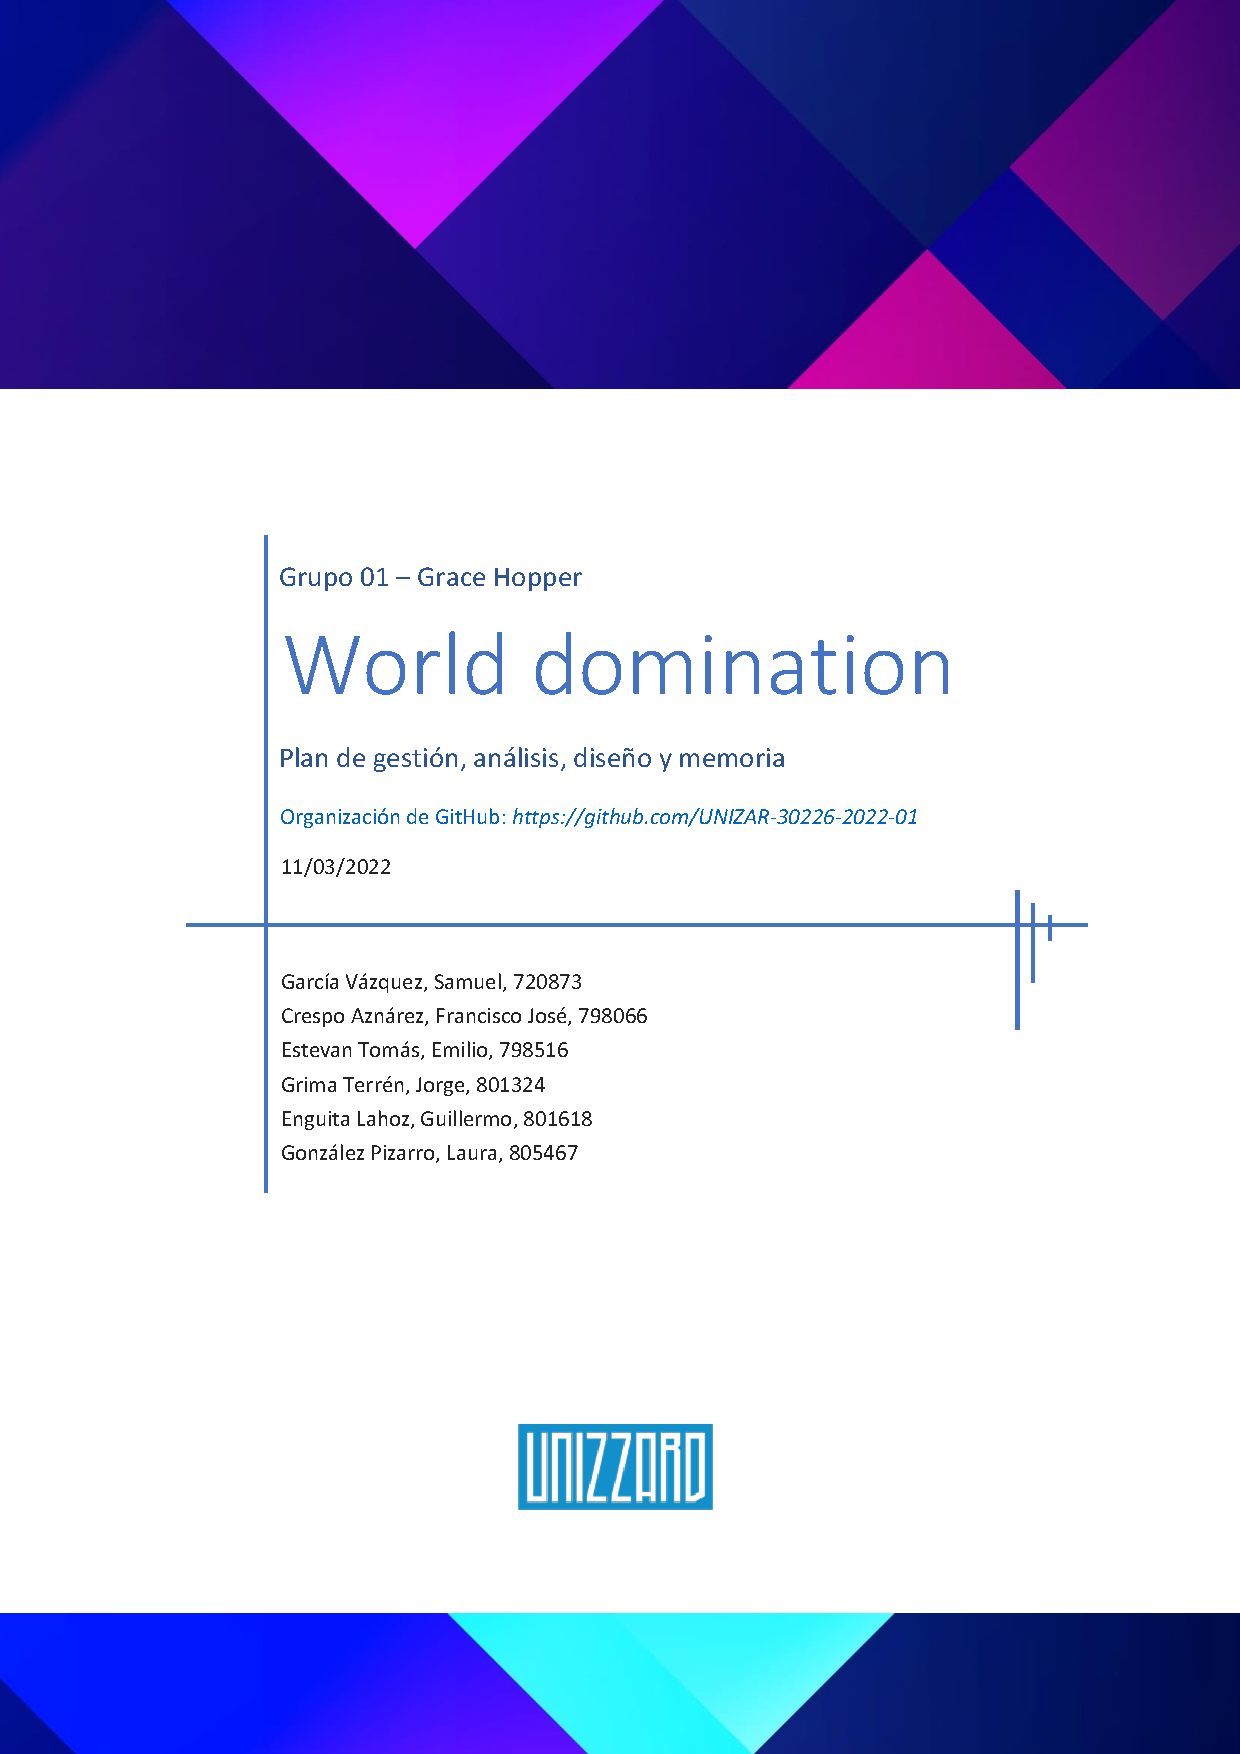
\includepdf[]{portadaMemoria.pdf}

\end{titlepage}
\newpage
%%%%%%%%%%%%%%%%%%%%%%%%%%%%%%%%%%%%%%%%%%%%%%%%%%%%%%%%%%%%%%%%%%%%%%%%%%%%%%%%%%%%%%%%%%%%%%%%





%%%%%%%%%%%%%%%%%%%%%%%%%%%%%%%%%%%%%%%%%%%%%%%%%%%%%%%%%%%%%%%%%%%%%%%%%%%%%%%%%%%%%%%%%%%%%%%%%
% CUERPO
%%%%%%%%%%%%%%%%%%%%%%%%%%%%%%%%%%%%%%%%%%%%%%%%%%%%%%%%%%%%%%%%%%%%%%%%%%%%%%%%%%%%%%%%%%%%%%%%
\thispagestyle{empty}
\fontsize{11pt}{11pt}\selectfont

\setcounter{tocdepth}{4}

% Índice con links en negro y no en azul
{
    \hypersetup{linkcolor=black}
    \doublespacing
    \tableofcontents
}

\thispagestyle{empty}

% Texto
\clearpage
\setcounter{page}{1}
\section{Introducción}
A lo largo del documento se va a presentar un proyecto que se ha denominado\textit{ \textbf{World Domination}}. Se trata de un juego de estrategia \textit{on-line} por turnos inspirado en \textit{Risk}, en el que cada jugador lucha contra el resto por la dominación del mundo. Cada uno de los jugadores cuenta con un número de soldados y territorios, así como con una baraja de cartas propia que podrán canjear por más soldados. En cada turno, los jugadores tendrán que luchar contra tropas bajo el dominio de los rivales, decidiéndose los resultados mediante tiradas de dados. \newline
%El sistema será capaz de gestionar las cuentas de los usuarios junto con las partidas que se desarrollen, así como la gestión de turnos y la inicialización y finalización de cada una de las partidas.

%Algunos de los objetivos fundamentales del sistema son:

%que constan de un \textit{email} y contraseña,%
Así mismo, el juego permitirá a los usuarios registrarse e iniciar sesión con sus credenciales, y el uso de una cuenta de usuario será necesario para jugar partidas. Gracias a que se almacenan cuentas de usuario, el sistema contará con una clasificación global de los mejores jugadores y de sus respectivas puntuaciones de las partidas jugadas. Por otro lado, el juego proporcionará funcionalidades adicionales que permitirán disfrutar de una experiencia social, fomentando la competición y una mayor participación en futuras partidas.\\ %Cada usuario podrá gestionar una lista de amigos.\\

Adicionalmente, los usuarios podrán personalizar elementos del juego en función de sus preferencias, como las fichas, su foto de perfil, o los dados usados durante las partidas, mediante puntos canjeables en la tienda del juego, que el sistema recompensará por haber jugado o ganado partidas. \\

Por otro lado, el juego permitirá crear partidas públicas y privadas, con contraseña, de 2 a 6 jugadores. Esto permitirá crear partidas entre grupos de amigos, o unirse a partidas públicas y conocer nuevos usuarios.\\

%Las partidas se desarrollarán de forma asíncrona, permitiendo a los usuarios responder en cualquier momento. Si el usuario se encuentra conectado, podrá ver una notificación en la pantalla. En el caso contrario, se enviará un correo al mismo notificando que puede realizar la jugada. Habrá un mecanismo de expulsión de jugadores que no respondan o realicen jugadas en un tiempo determinado. \\

A lo largo de la realización del proyecto se realizarán entregas parciales del trabajo llevado a cabo, en reuniones propuestas en unos plazos establecidos:

En primer lugar, se realizará una reunión para la evaluación parcial del sistema, con el objetivo de refinar requisitos y mostrar el progreso del desarrollo. Esto se realizará en la semana del 4 al 8 de Abril. \\

En segundo lugar, se realizará reunión para la evaluación de todas las funcionalidades del juego, con el sistema implementado en una versión final, con el objetivo de realizar ajustes finales. Esto se realizará en la semana del 16 al 20 de Mayo. \\

El sistema final se entregará no más tarde del 1 de junio, con los cambios propuestos durante las reuniones intermedias. \\

A continuación, se detallará la organización del proyecto, los equipos creados y sus objetivos, las tecnologías utilizadas,  y el calendario del proyecto con la división de las tareas asignadas a cada uno.
Además, realizaremos un análisis y diseño del sistema, y una revisión del transcurso del proyecto, desde el inicio hasta el cierre del mismo. \newpage

\section{Organización del proyecto}
El equipo está formado por 6 integrantes: Samuel García, Guillermo Enguita, Laura Gonzalez, Francisco Crespo, Emilio Estevan y Jorge Grima.
Hemos dividido el proyecto en tres bloques fundamentales:\newline
\begin{itemize}
    \item \textit{Backend} implementado con \textbf{Go} y desarrollo de la API, base de datos con \textit{PostgreSQL} y despliegue mediante \textit{Docker}.
    \item Primera versión del \textit{frontend} implementada con \textbf{React}.
    \item Segunda versión del \textit{frontend} implementada con \textbf{Angular}.\newline
\end{itemize}

El trabajo del primer bloque será llevado a cabo por Samuel y Guillermo, el del segundo bloque por Francisco y Emilio, mientras que el del tercer bloque será realizado por Laura y Jorge.
Aunque cada uno tenga un bloque asignado, en todo momento se ayudará a integrantes encargados del trabajo en otros bloques si fuera necesario. \newline

El equipo decidió nombrar como director a Francisco Crespo, será el portavoz y el encargado de tomar las decisiones más controvertidas, así como de realizar las entregas necesarias del trabajo.\newline

El responsable del control de configuraciones, construcción del software y aseguramiento de la calidad del producto será Samuel García.\\

La responsable de la división del trabajo, coordinación y la comunicación entre los miembros del proyecto será Laura González.

\section{Plan de gestión del proyecto}

A continuación, se describe cómo se llevaran a cabo distintas tareas a realizar en el proyecto: plan inicial de trabajo, división del trabajo a realizar o control de creación de software, entre otros.

\subsection{Inicio del proyecto}

Diversas tecnologías y lenguajes de programación utilizados en este proyecto eran, en un principio, desconocidos para los integrantes del equipo. Para solventar este problema, hemos tenido que realizar la siguiente formación común:

\begin{itemize}

\item Debido a que toda la documentación necesaria para el proyecto va a ser realizada en \textbf{Latex}, todos los miembros del equipo deberán adquirir conocimientos básicos para la utilización y explotación de esta herramienta. Para lograr este objetivo, realizaremos dos tutoriales. El primero de ellos, <<Learn LaTeX in 30 minutes>>\footnote{\href{https://www.overleaf.com/learn/latex/Learn_LaTeX_in_30_minutes}{\color{blue}{Learn LaTeX in 30 minutes}}}, se puede encontrar en la página web de \textit{Overleaf}. A su vez, seguiremos los manuales de ayuda proporcionados por la página oficial de \LaTeX \footnote{\href{https://latex-tutorial.com/tutorials/}{\color{blue}{Tutorial oficial de \LaTeX}}}.



\item Continuando lo anterior, los integrantes del Grupo 1 asistieron a la práctica: \textit{Puesta en marcha de GitHub y fundamentos de Git} impartida por los profesores de la asignatura \textit{Proyecto Software}, la cual consistió en familiarizarse con la herramienta \textbf{Git} y su uso en conjunto con \textbf{GitHub}. A su vez, por medio del tutorial: \textit{Git, GitHub y Publicación Web}\footnote{\href{https://github.com/flowsta/github}{\color{blue}{Git, GitHub y Publicación Web}}} se habían adquirido los conocimientos básicos de la misma.

\end{itemize}

Los grupos encargados de cada bloque del sistema realizaron formación específica. En primer lugar, los encargados del desarrollo del \textbf{backend} del sistema:

\begin{itemize}

\item Harán uso de \textbf{Go} como lenguaje de programación, al tener experiencia previa gracias a las prácticas de la asignatura de \textit{Sistemas Distribuidos}. De cara a fijar conocimientos y a aprender nuevas mecánicas, realizarán el tutorial de la página web oficial de \textbf{Go}.

\item A su vez, harán una formación relacionada con las distintas \textbf{API web}, concretamente el tutorial \textit{Introducción a las API web} de MozillaDeveloper\footnote{\href{https://developer.mozilla.org/es/docs/Learn/JavaScript/Client-side_web_APIs/Introduction}{\color{blue}{Introducción a las API web}}}.

\end{itemize}

Por otro lado, el equipo encargado del primer \textit{frontend}, implementado con \textbf{React}:

\begin{itemize}

\item  Este grupo realizará el tutorial oficial de \textbf{ReactJs}: \textit{Tutorial: Introducción a React}\footnote{\href{https://es.reactjs.org/tutorial/tutorial.html}{\color{blue}{Tutorial: Introducción a React}}}, que tiene una duración estimada de 8 horas. También harán el tutorial de API web anteriormente mencionado.

\end{itemize}

Por último, el equipo encargado de desarrollar el segundo \textit{frontend}, implementado con \textbf{Angular}:

\begin{itemize}

\item Realizará el tutorial \textit{Angular y TypeScript}\footnote{\href{https://angular.io/tutorial}{\color{blue}{Tutorial: Angular y TypeScript}}} proporcionado por \textit{DesarrolloWeb}, el cual tiene un tiempo estimado de realización próximo a las 7 horas.

\end{itemize}


\subsection{Control de configuraciones, construcción del software y aseguramiento de la calidad del producto}

Con el objetivo de tener una base de desarrollo, pruebas y objetivos de calidad comunes a todos los integrantes del grupo, se ha establecido una serie de normas a seguir durante el desarrollo del sistema.


%Todas estas normas son relativas a las tareas de construcción del \textit{software}, gestión de incidencias, automatización, calidad y despliegue del sistema por completo.

\subsubsection{Convenciones y procedimientos para la construcción y control del software}

Se han establecido las siguientes prácticas para mantener una configuración de proyectos y ficheros similar entre cada uno de los equipos del proyecto, bajo una serie de repositorios en \textit{Github}.

\begin{itemize}
    \item La organización y nombrado de los ficheros fuente seguirá las prácticas recomendadas por cada uno de los \textit{frameworks} a utilizar. De este modo, seguiremos las siguientes guías de estilo, nombrado de ficheros y organización de proyectos:
    \begin{itemize}
        \item Para \textbf{Angular}, utilizaremos la guía de estilo oficial\footnote{\href{https://angular.io/guide/styleguide}{\color{blue}{Guía de estilo oficial de Angular}}} y la guía de estructura de proyectos propuesta por la documentación oficial\footnote{\href{https://angular.io/guide/file-structure}{\color{blue}{Guía de estructura de proyectos oficial de Angular}}}.

        \item Para \textbf{React}, usaremos la
        guía de estilo de \textit{airbnb}\footnote{\href{https://airbnb.io/javascript/react/}{\color{blue}{Guía de estilo de React y Javascript de Airbnb}}} y la estructura de proyectos propuesta por la documentación oficial\footnote{\href{https://es.reactjs.org/docs/faq-structure.html}{\color{blue}{Guía de estructura de proyectos oficial de React}}}.

        \item Para \textbf{Go}, seguiremos el estilo impuesto por la herramienta automática de formato de dicho lenguaje\footnote{\href{https://pkg.go.dev/cmd/gofmt}{\color{blue}{Herramienta de formato y estilo oficial de golang}}} y la estructura de proyectos recomendada por la comunidad\footnote{\href{https://github.com/golang-standards/project-layout}{\color{blue}{Guía de estructura de proyectos recomendada para golang por la comunidad}}}.
    \end{itemize}

    \item Todo el código será subido a los repositorios de la organización de \textit{Github}\footnote{\href{https://github.com/UNIZAR-30226-2022-01}{\color{blue}{Repositorio de la organización de \textit{Github}}}}, donde todos los miembros tendrán permisos de acceso, modificación y administración de los mismos. Los repositorios serán los siguientes:
    \begin{itemize}
        \item Un repositorio para el \textit{backend} del sistema (\textbf{API})\footnote{\href{https://github.com/UNIZAR-30226-2022-01/proyecto_software_backend}{\color{blue}{Repositorio del \textit{backend} del sistema}}}.

        \item Un repositorio para el \textit{frontend} de \textbf{React}\footnote{\href{https://github.com/UNIZAR-30226-2022-01/proyecto_software_frontend_react}{\color{blue}{Repositorio del frontend de \textit{React}}}}.

        \item Un repositorio para el \textit{frontend} de \textbf{Angular}\footnote{\href{https://github.com/UNIZAR-30226-2022-01/proyecto_software_frontend_angular}{\color{blue}{Repositorio del frontend de \textit{Angular}}}}.

        \item Un repositorio para la documentación\footnote{\href{https://github.com/UNIZAR-30226-2022-01/proyecto_software_documentacion}{\color{blue}{Repositorio de documentación}}}, en el cual se localizarán todos los archivos de documentación interna y de cara al usuario, ya estén terminados como archivos .pdf o en construcción, como archivos de \LaTeX.
    \end{itemize}


\end{itemize}

\subsubsection{Convenciones y procedimientos para el despliegue del software}

Con el objetivo de proveer un despliegue homogéneo del proyecto, tanto para las pruebas durante el desarrollo como para las entregas al cliente, se han establecido los siguientes puntos.

\begin{itemize}
    \item Las herramientas necesarias para construir el \textit{software} serán aquellas necesarias para compilar los \textit{frontend} de \textbf{React} y \textbf{Angular} y el \textit{backend} de \textbf{Go} por separado, junto a \textbf{Docker} y \textbf{Docker-compose}. \newline

    Con el objetivo de tener una base de pruebas y desarrollo uniforme, en el repositorio de backend se porporcionarán los siguientes scripts de automatización:
    \begin{itemize}
        \item Dos grupos de scripts de automatización de despliegue de los frontend \textbf{React} y \textbf{Angular} por separado, que crean un contenedor de Docker con el servidor web sirviendo uno de los frontend.

        \item Un grupo de scripts de automatización del \textbf{backend}, que ponen en marcha un par de contenedores ligados mediante \textit{docker-compose} para el servidor de \textit{API} y la base de datos respectivamente.
    \end{itemize}

    Los contenedores de \textit{frontend} serán capaces de comunicarse con los de \textit{backend} mediante ligado de puertos en la máquina host. Durante el desarrollo del sistema, ambos grupos de contenedores se comunicarán en la propia máquina del desarrollador, y para el despliegue se adaptarán tanto las direcciones a utilizar en el código como los puertos en los archivos de despliegue de \textit{Docker}.

    Los \textit{scripts} de automatización se harán cargo de la compilación, obtención de dependencias y puesta en marcha y configuración de cualquier elemento adicional como la base de datos, haciendo posible desplegar un entorno de pruebas común.

    \item El despliegue en entornos de producción se realizará con contenedores de \textbf{Docker} en la infraestructura en la nube de \textbf{Google Cloud}, de tal forma que cada equipo en la nube corresponderá al despliegue en contenedores de cada uno de los \textit{frontend} y del \textit{backend}. Por motivos de seguridad, las claves de acceso a la base de datos o rutas y puertos a utilizar serán establecidas por el cliente e introducidas en los contenedores mediante un fichero de variables de entorno.
\end{itemize}

\subsubsection{Convenciones y procedimientos para el control de la calidad del software}

Debido a que se van a utilizar diferentes lenguajes de programación y \textit{frameworks} en cada una de las partes del proyecto, se han establecido una serie de prácticas comunes a seguir. También se ha planteado una estrategia de pruebas manuales y automáticas, para poder medir y controlar la calidad del software.

\begin{itemize}
    \item Se seguirán buenas prácticas para la documentación del código. En concreto, se seguirán las publicadas por \textit{Google}\footnote{\href{https://developers.google.com/style/api-reference-comments}{\color{blue}{\textit{Guía de documentacion para desarrolladores de Google}}}} para la documentación de la \textit{API} pública.

    \item Debido a que se ha acordado que el diseño de la interfaz deberá ser lo más similar posible entre ambos \textit{frontend} para mantener la consistencia, se comprobará la implementación de cada pantalla en el otro \textit{frontend}, si ya lo está. Así mismo, se comunicarán derivaciones importantes respecto al diseño de pantallas inicial.
    
    Las inconsistencias de diseño encontradas se deberán comunicar al otro equipo, y se acordará una solución a las mismas.
    
    \item Tras añadir una nueva funcionalidad, el encargado de su implementación comprobará su corrección, realizando pruebas manuales y automáticas. Para ello, seguiremos la siguiente estrategia:
    \begin{itemize}
        \item El \textit{backend} proporcionará un conjunto de pruebas automáticas sobre cada uno de los elementos de la \textit{API}, utilizando las herramientas de \textit{testing} de \textit{Go}.

        Tras añadir una nueva funcionalidad a la \textit{API}, garantizaremos que se pasen todas las pruebas automáticas antes de persistir los cambios.

        \item Cada uno de los equipos de \textit{frontend} realizará pruebas exploratorias a la hora de implementar funcionalidades que involucren a la \textit{API}, teniendo la garantía de que ha pasado las pruebas automáticas previamente.
        \end{itemize}


    \item Las entregas a los clientes serán probadas íntegramente, por todos los miembros del equipo, para garantizar que no existen problemas en las funcionalidades implementadas hasta dicho momento.

    La estrategia de pruebas previas a la entrega será la realización, durante una reunión entre todos los miembros del equipo, de una prueba exploratoria común sobre ambos \textit{frontend} al mismo tiempo. Esta prueba buscará confirmar que todos los requisitos establecidos han sido implementados correctamente, realizando las acciones necesarias para comprobar cada uno de los requisitos de la lista. \\

    Esta prueba se realizará de tal forma que cada equipo de \textit{frontend} pruebe las funcionalidades sobre el que no ha desarrollado, para favorecer encontrar errores e inconsistencias inesperadas. Por otro lado, cada miembro original del equipo de \textit{backend} realizará la prueba sobre el \textit{frontend} \textit{React} y otro sobre \textit{Angular}, comprobando también que las interacciones con la \textit{API} son correctas.

    Una vez realizada la prueba, los resultados se comunicarán al responsable de estos aspectos, que coordinará la corrección de los errores observados. Si se considera que han aparecido un gran número de errores e inconsistencias, se repetirá el proceso de prueba una vez corregidas.
\end{itemize}


\subsection{Calendario del proyecto, división del trabajo, coordinación, comunicaciones, monitorización y seguimiento}

%%%%%%%%%%%%%%%%%%%%%%%%%%%%%%%
%%%%%%%%%%%%%%%%%%%%%%%%%%%%%%%
%%%%%%%%%%%%%%%%%%%%%%%%%%%%%%%
%%%%%%%%%%%%%%%%%%%%%%%%%%%%%%%%%%%%%%%%%%%%%%%%%%%%%%%%%%%
% De control de configuraciones y software, a incluir en comunicaciones:
%%%%%%%%%%%%%%%%%%%%%%%%%%%%%%%%%%%%%%%%%%%%%%%%%%%%%%%%%%%

\subsubsection{Coordinación entre equipos}
Con el objetivo de favorecer la coordinación entre los equipos y la visibilidad y monitorización de las tareas realizadas, se han establecido las siguientes normas:\\

La gestión de incidencias y tareas pendientes se realizará mediante el gestor de incidencias de \textbf{GitHub} del repositorio relacionado con ellas. Debido a que no permite crear incidencias que abarquen múltiples repositorios, cada uno de ellos tendrá las incidencias globales que afecten a varios de ellos replicadas. \\

Todas las tareas, funcionalidades a implementar o ampliar y errores a arreglar serán documentados en incidencias individuales con una descripción concisa. Estas formarán parte de hitos para entregas y versiones intermedias si aplica. Las incidencias se clasificarán utilizando etiquetas. De la misma forma que con las incidencias, los hitos globales estarán replicados en cada repositorio con las tareas e incidencias correspondientes. \\

Las incidencias serán asignadas a quienes trabajen en ella para mantener un control de actividades y tiempo, y podrán ser cerradas y abiertas de nuevo libremente. \\

Todos los \textit{commits} a realizar no requerirán aprobación, pero deberán ser probados para que no causen problemas de compilación, y deberían ser tan funcionalmente completos como sea posible. Además, no deberán abarcar un número excesivo de cambios en el código para favorecer que se puedan deshacer si es necesario, y deberán tener una descripción concisa de las modificaciones realizadas. \\

Por ello, se han establecido los siguientes objetivos a comprobar cada vez que se realiza un \textit{commit}:
\begin{itemize}
    \item Se comprobará que el código compila tras implementar dicho \textit{commit}, y que todos los test automáticos implementados hasta el momento siguen siendo correctos.
    \item El ámbito del \textit{commit} no deberá abarcar más allá del grupo de tareas de una incidencia en concreto a no ser que no sea posible evitarlo. Esto ayuda a evitar realizar un número excesivo de cambios.
    \item Los \textit{commits} no deberán exceder de 500 nuevas líneas siempre que sea posible, excluyendo la subida de ficheros o implementaciones de funciones inherentemente largas, como los test automáticos.
\end{itemize}


%%%%%%%%%%%%%%%%%%%%%%%%%%%%%%%
%%%%%%%%%%%%%%%%%%%%%%%%%%%%%%%
%%%%%%%%%%%%%%%%%%%%%%%%%%%%%%%
%%%%%%%%%%%%%%%%%%%%%%%%%%%%%%%
%%%%%%%%%%%%%%%%%%%%%%%%%%%%%%%
%%%%%%%%%%%%%%%%%%%%%%%%%%%%%%%
\subsubsection{Seguimiento de objetivos}
La coordinación y seguimiento de objetivos del proyecto se va a seguir mediante un diagrama de \textit{Gantt}, apreciable en la Figura \ref{fig:gantt}, el cual podrá ser modificado en el futuro debido a posibles adelantos o retrasos en alguna de las tareas, y también por tareas imprevistas que pueden surgir durante la realización del proyecto.\\

\begin{landscape}
    \pagestyle{empty}
    \begin{figure}[!p]
    \centering

    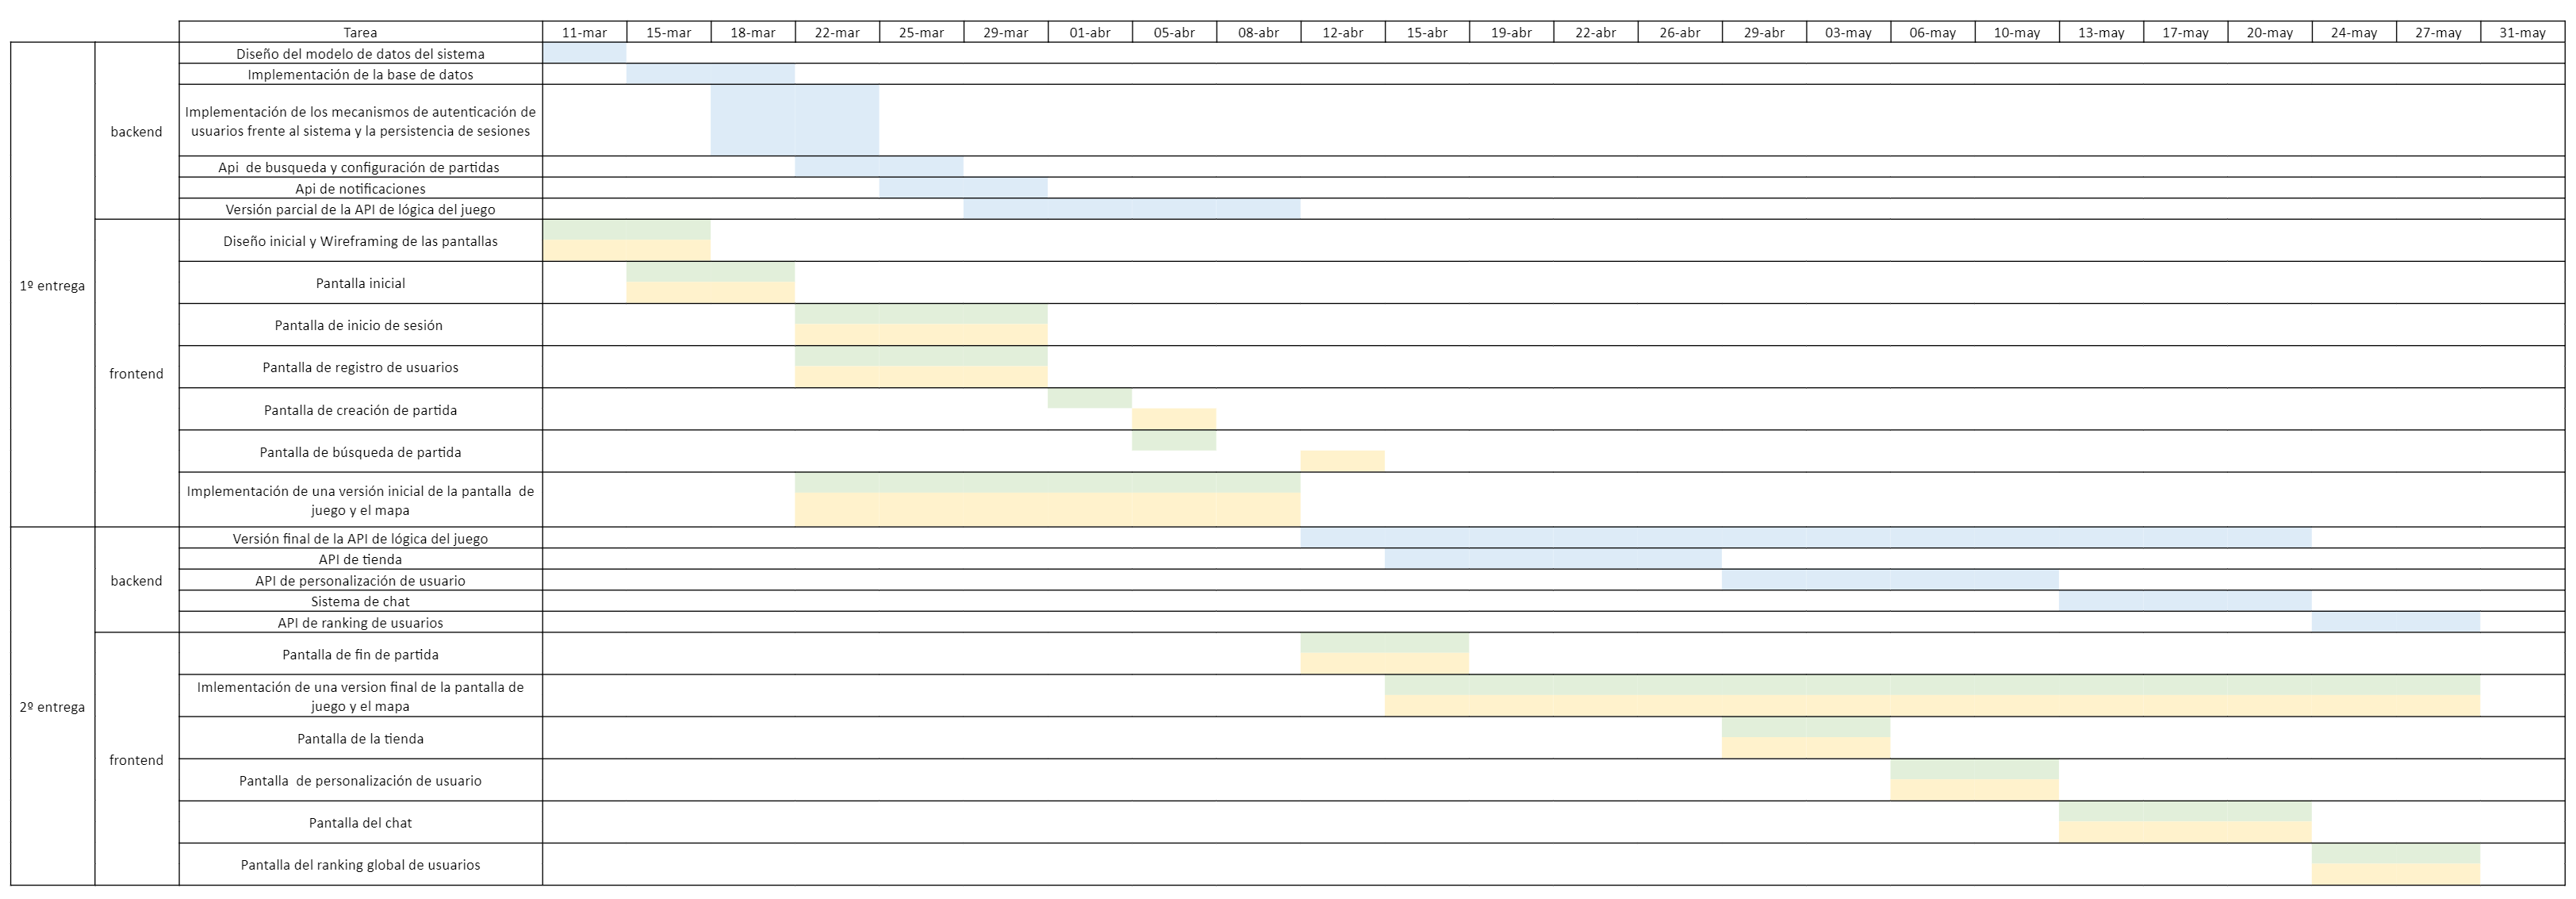
\includegraphics[width=1.7\textwidth]{diagramas/gantt.png}
    \caption{Diagrama de Gantt.}
    \label{fig:gantt}
\end{figure}
\end{landscape}

 Para el diseño de las pantallas se realizó un boceto simple de estas, el cual se tomará como referencia en mayor medida por ambos \texit{frontend}.\footnote{\href{https://github.com/UNIZAR-30226-2022-01/proyecto_software_documentacion/tree/main/imagenes}{\color{blue}{\textit{Diseño inicial}}}}.
\\

La división de tareas diarias internas en cada uno de los equipos se consensuará entre sus miembros, y se preferirá en todo momento la programación por pares.\\

Tanto el \textit{frontend} como el \textit{backend} poseerán un calendario de seguimiento propio en el cual se establecen los objetivos a realizar junto a sus fechas limite para ser completadas. \\

Ambos tienen en común dos fechas las son \textbf{8 de abril} debido a que esta es la es la entrega intermedia, en donde se le mostrará al cliente una primera versión funcional del proyecto
y \textbf{30 de junio} porque esta es la fecha de la entrega del proyecto.\\

Cada dos semanas todos los miembros del equipo rellenarán un cuestionario indicando las horas trabajadas y el progreso realizado. Por otro lado las actas se tomarán por turnos durante las reuniones con el cliente en las fechas indicadas por él mismo.\\

Las métricas de rendimiento del equipo irán marcadas por el estado por cada una de las incidencias y tareas pendientes de cada uno de los repositorios. Si se diese el caso de que algún equipo quedase rezagado respecto al resto o sufriera algún imprevisto, éste deberá comentárselo al coordinador del equipo para que así se pueda tomar una decisión sobre cómo actuar al respecto.

\subsubsection{Calendario de seguimiento para el frontend}
El calendario interno para el \textit{frontend} va a ser el mismo para ambas implementaciones. La tabla \ref{table:frontend} muestra las tareas a realizar por este equipo. \newline

\subsubsection{Calendario de seguimiento para el backend}
 La tabla \ref{table:backend} muestra las tareas a realizar por el equipo. \newline

% Please add the following required packages to your document preamble:
% \usepackage{multirow}
\begin{landscape}
\pagestyle{empty}
\begin{table}[hbt!]
\small
\centering
\begin{tabular}{c|ccll|cc|}
\cline{2-7}
\multirow{2}{*}{}                                 & \multicolumn{4}{c|}{\multirow{2}{*}{Tarea}}                                                                                                                                                                                      & \multicolumn{2}{c|}{Personas asignadas}                                      \\ \cline{6-7}
                                                  & \multicolumn{4}{c|}{}                                                                                                                                                                                                            & \multicolumn{1}{c|}{Angular}                & \multicolumn{1}{l|}{React}     \\ \hline
\multicolumn{1}{|c|}{\multirow{14}{*}{Entrega 1}} & \multicolumn{4}{c|}{Pantalla inicial}                                                                                                                                                                                            & \multicolumn{1}{c|}{Jorge y Laura}          & \multirow{9}{*}{Emilio y Fran} \\ \cline{2-6}
\multicolumn{1}{|c|}{}                            & \multicolumn{1}{c|}{\multirow{2}{*}{Pantalla de registro de usuario}}                                           & \multicolumn{3}{c|}{Diseño del HTML y CSS}                                                                     & \multicolumn{1}{c|}{Jorge y Laura}          &                                \\ \cline{3-6}
\multicolumn{1}{|c|}{}                            & \multicolumn{1}{c|}{}                                                                                           & \multicolumn{3}{c|}{Conexión con la API}                                                                       & \multicolumn{1}{c|}{Laura}                  &                                \\ \cline{2-6}
\multicolumn{1}{|c|}{}                            & \multicolumn{1}{c|}{\multirow{2}{*}{Pantalla de inicio de sesión}}                                              & \multicolumn{3}{c|}{Diseño del HTML y CSS}                                                                     & \multicolumn{1}{c|}{Jorge y Laura}          &                                \\ \cline{3-6}
\multicolumn{1}{|c|}{}                            & \multicolumn{1}{c|}{}                                                                                           & \multicolumn{3}{c|}{Conexión con la API}                                                                       & \multicolumn{1}{c|}{Laura}                  &                                \\ \cline{2-6}
\multicolumn{1}{|c|}{}                            & \multicolumn{1}{c|}{\multirow{2}{*}{Pantalla de crear de partida}}                                              & \multicolumn{3}{c|}{Diseño del HTML y CSS}                                                                     & \multicolumn{1}{c|}{\multirow{2}{*}{Laura}} &                                \\ \cline{3-5}
\multicolumn{1}{|c|}{}                            & \multicolumn{1}{c|}{}                                                                                           & \multicolumn{3}{c|}{Conexión con la API}                                                                       & \multicolumn{1}{c|}{}                       &                                \\ \cline{2-6}
\multicolumn{1}{|c|}{}                            & \multicolumn{1}{c|}{\multirow{2}{*}{Pantalla de búsqueda de partidas}}                                          & \multicolumn{3}{c|}{Diseño del HTML y CSS}                                                                     & \multicolumn{1}{c|}{\multirow{2}{*}{Jorge}} &                                \\ \cline{3-5}
\multicolumn{1}{|c|}{}                            & \multicolumn{1}{c|}{}                                                                                           & \multicolumn{3}{c|}{Conexión con la API}                                                                       & \multicolumn{1}{c|}{}                       &                                \\ \cline{2-7}
\multicolumn{1}{|c|}{}                            & \multicolumn{1}{c|}{\multirow{5}{*}{Implementación de una versión inicial de la pantalla del juego y del mapa}} & \multicolumn{3}{c|}{Diseño del mapa}                                                                           & \multicolumn{2}{c|}{Emilio, Fran, Jorge y Laura}                             \\ \cline{3-7}
\multicolumn{1}{|c|}{}                            & \multicolumn{1}{c|}{}                                                                                           & \multicolumn{3}{c|}{Mapa auxiliar}                                                                             & \multicolumn{2}{c|}{Fran}                                                    \\ \cline{3-7}
\multicolumn{1}{|c|}{}                            & \multicolumn{1}{c|}{}                                                                                           & \multicolumn{3}{c|}{Representación de usuarios}                                                                & \multicolumn{2}{c|}{Emilio}                                                  \\ \cline{3-7}
\multicolumn{1}{|c|}{}                            & \multicolumn{1}{c|}{}                                                                                           & \multicolumn{3}{c|}{Botones del mapa}                                                                          & \multicolumn{2}{c|}{Fran}                                                    \\ \cline{3-7}
\multicolumn{1}{|c|}{}                            & \multicolumn{1}{c|}{}                                                                                           & \multicolumn{3}{c|}{Diseño de las top-bar y bottom-bar}                                                        & \multicolumn{2}{c|}{Laura}                                                   \\ \hline
\multicolumn{1}{|c|}{\multirow{22}{*}{Entrega 2}} & \multicolumn{1}{c|}{\multirow{8}{*}{Implementación de la versión final de la pantalla del juego y del mapa}}    & \multicolumn{3}{c|}{Diseño de los dados}                                                                       & \multicolumn{2}{c|}{\multirow{22}{*}{Por determinar}}                        \\ \cline{3-5}
\multicolumn{1}{|c|}{}                            & \multicolumn{1}{c|}{}                                                                                           & \multicolumn{3}{c|}{Diseño de las cartas}                                                                      & \multicolumn{2}{c|}{}                                                        \\ \cline{3-5}
\multicolumn{1}{|c|}{}                            & \multicolumn{1}{c|}{}                                                                                           & \multicolumn{3}{c|}{Diseño de atacar a un pais}                                                                & \multicolumn{2}{c|}{}                                                        \\ \cline{3-5}
\multicolumn{1}{|c|}{}                            & \multicolumn{1}{c|}{}                                                                                           & \multicolumn{3}{c|}{Diseño de movimientos de tropas}                                                           & \multicolumn{2}{c|}{}                                                        \\ \cline{3-5}
\multicolumn{1}{|c|}{}                            & \multicolumn{1}{c|}{}                                                                                           & \multicolumn{3}{c|}{\begin{tabular}[c]{@{}c@{}}Diseño de componente de información \\ de usuario\end{tabular}} & \multicolumn{2}{c|}{}                                                        \\ \cline{3-5}
\multicolumn{1}{|c|}{}                            & \multicolumn{1}{c|}{}                                                                                           & \multicolumn{3}{c|}{Diseño del battle log}                                                                     & \multicolumn{2}{c|}{}                                                        \\ \cline{3-5}
\multicolumn{1}{|c|}{}                            & \multicolumn{1}{c|}{}                                                                                           & \multicolumn{3}{c|}{Diseño de ayuda del mapa}                                                                  & \multicolumn{2}{c|}{}                                                        \\ \cline{3-5}
\multicolumn{1}{|c|}{}                            & \multicolumn{1}{c|}{}                                                                                           & \multicolumn{3}{c|}{Diseño de canjeo de cartas}                                                                & \multicolumn{2}{c|}{}                                                        \\ \cline{2-5}
\multicolumn{1}{|c|}{}                            & \multicolumn{1}{c|}{\multirow{2}{*}{Pantalla del perfil de usuario}}                                            & \multicolumn{3}{c|}{Diseño del HTML y CSS}                                                                     & \multicolumn{2}{c|}{}                                                        \\ \cline{3-5}
\multicolumn{1}{|c|}{}                            & \multicolumn{1}{c|}{}                                                                                           & \multicolumn{3}{c|}{Conexión con la API}                                                                       & \multicolumn{2}{c|}{}                                                        \\ \cline{2-5}
\multicolumn{1}{|c|}{}                            & \multicolumn{1}{c|}{\multirow{2}{*}{Pantalla del buzón de notificaciones del usuario}}                          & \multicolumn{3}{c|}{Diseño del HTML y CSS}                                                                     & \multicolumn{2}{c|}{}                                                        \\ \cline{3-5}
\multicolumn{1}{|c|}{}                            & \multicolumn{1}{c|}{}                                                                                           & \multicolumn{3}{c|}{Conexión con la API}                                                                       & \multicolumn{2}{c|}{}                                                        \\ \cline{2-5}
\multicolumn{1}{|c|}{}                            & \multicolumn{1}{c|}{\multirow{2}{*}{Pantalla de fin de partida}}                                                & \multicolumn{3}{c|}{Diseño del HTML y CSS}                                                                     & \multicolumn{2}{c|}{}                                                        \\ \cline{3-5}
\multicolumn{1}{|c|}{}                            & \multicolumn{1}{c|}{}                                                                                           & \multicolumn{3}{c|}{Conexión con la API}                                                                       & \multicolumn{2}{c|}{}                                                        \\ \cline{2-5}
\multicolumn{1}{|c|}{}                            & \multicolumn{1}{c|}{\multirow{2}{*}{Pantalla de la tienda}}                                                     & \multicolumn{3}{c|}{Diseño del HTML y CSS}                                                                     & \multicolumn{2}{c|}{}                                                        \\ \cline{3-5}
\multicolumn{1}{|c|}{}                            & \multicolumn{1}{c|}{}                                                                                           & \multicolumn{3}{c|}{Conexión con la API}                                                                       & \multicolumn{2}{c|}{}                                                        \\ \cline{2-5}
\multicolumn{1}{|c|}{}                            & \multicolumn{1}{c|}{\multirow{2}{*}{Pantalla de personalización de usuario}}                                    & \multicolumn{3}{c|}{Diseño del HTML y CSS}                                                                     & \multicolumn{2}{c|}{}                                                        \\ \cline{3-5}
\multicolumn{1}{|c|}{}                            & \multicolumn{1}{c|}{}                                                                                           & \multicolumn{3}{c|}{Conexión con la API}                                                                       & \multicolumn{2}{c|}{}                                                        \\ \cline{2-5}
\multicolumn{1}{|c|}{}                            & \multicolumn{1}{c|}{\multirow{2}{*}{Pantalla del chat en la partida}}                                           & \multicolumn{3}{c|}{Diseño del HTML y CSS}                                                                     & \multicolumn{2}{c|}{}                                                        \\ \cline{3-5}
\multicolumn{1}{|c|}{}                            & \multicolumn{1}{c|}{}                                                                                           & \multicolumn{3}{c|}{Conexión con la API}                                                                       & \multicolumn{2}{c|}{}                                                        \\ \cline{2-5}
\multicolumn{1}{|c|}{}                            & \multicolumn{1}{c|}{\multirow{2}{*}{Pantalla de la clasificación global de usuarios}}                           & \multicolumn{3}{c|}{Diseño del HTML y CSS}                                                                     & \multicolumn{2}{c|}{}                                                        \\ \cline{3-5}
\multicolumn{1}{|c|}{}                            & \multicolumn{1}{c|}{}                                                                                           & \multicolumn{3}{c|}{Conexión con la API}                                                                       & \multicolumn{2}{c|}{}                                                        \\ \hline
\end{tabular}
\caption{Tabla de esfuerzos del frontend}
\label{table:frontend}
\end{table}
\end{landscape}
%\end{center}
\FloatBarrier

\newpage

\begin{landscape}
\pagestyle{empty}
\begin{table}[hbt!]
\small
\centering
\begin{tabular}{c|cc|c|}
\cline{2-4}
                                                   & \multicolumn{2}{c|}{Tarea}                                                                                                                                                                                                                                                                                                        & Personas asignada                   \\ \hline
\multicolumn{1}{|c|}{\multirow{25}{*}{2º entrega}} & \multicolumn{2}{c|}{Diseño del modelo de datos del sistema}                                                                                                                                                                                                                                                                       & Samuel y Guillermo                  \\ \cline{2-4}
\multicolumn{1}{|c|}{}                             & \multicolumn{2}{c|}{Implementación de la base de datos}                                                                                                                                                                                                                                                                           & Samuel y Guillermo                  \\ \cline{2-4}
\multicolumn{1}{|c|}{}                             & \multicolumn{2}{c|}{\begin{tabular}[c]{@{}c@{}}Implementación de los mecansimos de autenticación \\ de usuarios frente al sistema y persistencia de sesiones\end{tabular}}                                                                                                                                                        & Samuel y Guillermo                  \\ \cline{2-4}
\multicolumn{1}{|c|}{}                             & \multicolumn{1}{c|}{\multirow{6}{*}{\begin{tabular}[c]{@{}c@{}}API de búsqueda y \\ configuración de partidas\end{tabular}}}   & Búsqueda de partidas                                                                                                                                                                             & \multirow{5}{*}{Samuel y Guillermo} \\ \cline{3-3}
\multicolumn{1}{|c|}{}                             & \multicolumn{1}{c|}{}                                                                                                          & Creación de partidas                                                                                                                                                                             &                                     \\ \cline{3-3}
\multicolumn{1}{|c|}{}                             & \multicolumn{1}{c|}{}                                                                                                          & Documentar búsqueda de partidas                                                                                                                                                                  &                                     \\ \cline{3-3}
\multicolumn{1}{|c|}{}                             & \multicolumn{1}{c|}{}                                                                                                          & Documentar creación de partidas                                                                                                                                                                  &                                     \\ \cline{3-3}
\multicolumn{1}{|c|}{}                             & \multicolumn{1}{c|}{}                                                                                                          & Unirse a partidas                                                                                                                                                                                &                                     \\ \cline{3-4}
\multicolumn{1}{|c|}{}                             & \multicolumn{1}{c|}{}                                                                                                          & Abandonar partidas                                                                                                                                                                               & Samuel                              \\ \cline{2-4}
\multicolumn{1}{|c|}{}                             & \multicolumn{2}{c|}{API de notificaciones}                                                                                                                                                                                                                                                                                        & Samuel                              \\ \cline{2-4}
\multicolumn{1}{|c|}{}                             & \multicolumn{1}{c|}{\multirow{5}{*}{\begin{tabular}[c]{@{}c@{}}Versión parcial de la API de \\ lógica del juego\end{tabular}}} & Crear autómata de una partida                                                                                                                                                                    & \multirow{4}{*}{Samuel y Guillermo} \\ \cline{3-3}
\multicolumn{1}{|c|}{}                             & \multicolumn{1}{c|}{}                                                                                                          & Definir acciones a realizar                                                                                                                                                                      &                                     \\ \cline{3-3}
\multicolumn{1}{|c|}{}                             & \multicolumn{1}{c|}{}                                                                                                          & Definir el estado de una partida                                                                                                                                                                 &                                     \\ \cline{3-3}
\multicolumn{1}{|c|}{}                             & \multicolumn{1}{c|}{}                                                                                                          & Definir endponits de API para consultar cada elemento de la partida                                                                                                                              &                                     \\ \cline{3-4}
\multicolumn{1}{|c|}{}                             & \multicolumn{1}{c|}{}                                                                                                          & Definir endpoints de API para acciones de la partida                                                                                                                                             & Samuel                              \\ \cline{2-4}
\multicolumn{1}{|c|}{}                             & \multicolumn{1}{c|}{\multirow{2}{*}{API auxiliares}}                                                                           & Listar amigos                                                                                                                                                                                    & \multirow{2}{*}{Guillermo}          \\ \cline{3-3}
\multicolumn{1}{|c|}{}                             & \multicolumn{1}{c|}{}                                                                                                          & Obtener información de perfil de usuario                                                                                                                                                         &                                     \\ \cline{2-4}
\multicolumn{1}{|c|}{}                             & \multicolumn{1}{c|}{\multirow{7}{*}{Implementación del principio de la partida}}                                               & Función de poblado aleatorio del mapa                                                                                                                                                            & \multirow{7}{*}{Samuel}             \\ \cline{3-3}
\multicolumn{1}{|c|}{}                             & \multicolumn{1}{c|}{}                                                                                                          & Función de roll de dados                                                                                                                                                                         &                                     \\ \cline{3-3}
\multicolumn{1}{|c|}{}                             & \multicolumn{1}{c|}{}                                                                                                          & Función de selección de primer usuario de una partida y siguientes                                                                                                                               &                                     \\ \cline{3-3}
\multicolumn{1}{|c|}{}                             & \multicolumn{1}{c|}{}                                                                                                          & Función de inicio de partida                                                                                                                                                                     &                                     \\ \cline{3-3}
\multicolumn{1}{|c|}{}                             & \multicolumn{1}{c|}{}                                                                                                          & Endpoint de obtener la lista de acciones para un usuario y su indice de la lista actual                                                                                                          &                                     \\ \cline{3-3}
\multicolumn{1}{|c|}{}                             & \multicolumn{1}{c|}{}                                                                                                          & Endpoint de reforzar territorio                                                                                                                                                                  &                                     \\ \cline{3-3}
\multicolumn{1}{|c|}{}                             & \multicolumn{1}{c|}{}                                                                                                          & \begin{tabular}[c]{@{}c@{}}Test unitarios de comprobación de almacen de partidas, inicio de una partida \\ tras alcanzar maxJugadores, acciones y obtención de la lista de acciones\end{tabular} &                                     \\ \cline{2-4}
\multicolumn{1}{|c|}{}                             & \multicolumn{2}{c|}{Implementación de la fase de ataque}                                                                                                                                                                                                                                                                          & Guillermo                           \\ \hline
\multicolumn{1}{|c|}{\multirow{6}{*}{2º entrega}}  & \multicolumn{2}{c|}{API de ranking}                                                                                                                                                                                                                                                                                               & \multirow{6}{*}{Por determinar}     \\ \cline{2-3}
\multicolumn{1}{|c|}{}                             & \multicolumn{2}{c|}{API de personalización de perfiles de usuario}                                                                                                                                                                                                                                                                &                                     \\ \cline{2-3}
\multicolumn{1}{|c|}{}                             & \multicolumn{2}{c|}{API de tienda}                                                                                                                                                                                                                                                                                                &                                     \\ \cline{2-3}
\multicolumn{1}{|c|}{}                             & \multicolumn{2}{c|}{Implementación de la fase de fortiticación}                                                                                                                                                                                                                                                                   &                                     \\ \cline{2-3}
\multicolumn{1}{|c|}{}                             & \multicolumn{2}{c|}{Implementación de la fase de fortificación}                                                                                                                                                                                                                                                                   &                                     \\ \cline{2-3}
\multicolumn{1}{|c|}{}                             & \multicolumn{2}{c|}{API de notificaciones}                                                                                                                                                                                                                                                                                        &                                     \\ \hline
\end{tabular}
\caption{Tabla de esfuerzos del backend}
\label{table:backend}
\end{table}
\end{landscape}
\FloatBarrier

\section{Análisis y diseño del sistema}

\subsection{Análisis de requisitos}
Los requisitos funcionales de nuestra aplicación se pueden encontrar detallados en la tabla \ref{tab:rf}. La tabla \ref{tab:rnf} recoge los requisitos no funcionales. Ambos tipos de requisitos se encuentran claramente detallados e identificados, para facilitar su referencia en documentación futura.
\renewcommand{\arraystretch}{1.3}\\
\begin{longtable}[h!]{| p{.10\textwidth} | p{.90\textwidth} |}
    \caption{Requisitos funcionales de la aplicación.}
    \label{tab:rf}
    \centering
        \hline
         Código & Descripción  \\
         \hline
         RF-1 & El sistema permitirá a los usuarios registrarse, utilizando un correo electrónico y estableciendo un nombre de usuario y una contraseña.\\
         \hline
         RF-2 & El sistema permitirá a los usuarios iniciar sesión, utilizando su nombre de usuario y su contraseña.\\
         \hline
         RF-3 & El sistema proporcionará a los usuarios un juego de \textit{Risk}.\\
         \hline
         RF-3.1 & Al comenzar la partida, se distribuirán equitativamente los territorios de manera aleatoria.\\
         \hline
         RF-3.2 & Cada turno de juego dispondrá de las siguiente fases: Refuerzo, Ataque y Fortificación. \\
         \hline
         RF-3.3 & Al empezar el turno del jugador, se le otorgará un número de ejércitos en función del número de territorios y continentes que ocupe.\\
         \hline
         RF-3.4 & Durante la fase de refuerzo, el jugador deberá colocar todas sus tropas distribuyéndolas como desee entre los territorios que domine.\\
         \hline
         RF-3.5 & El jugador podrá cambiar un conjunto de 3 cartas para recibir ejércitos durante la fase de refuerzo.\\
         \hline
         RF-3.6 & El jugador recibirá una carta al final del turno, si durante dicho turno ha conquistado algún territorio.\\
         \hline
         RF-3.7 & Las cartas pueden ser de 4 tipos: infantería, caballería, artillería y comodines.
         Además, cada carta tendrá un territorio asignado (excepto los comodines).\\
         \hline
         RF-3.8 & Para que un cambio de cartas sea válido, se deberán cambiar 3 cartas del mismo tipo, dos del mismo tipo junto a un comodín o una carta de cada tipo. \\
         \hline
         RF-3.9 & El número de ejércitos recibidos por cada cambio dependerá del número de cambios realizados. El primer cambio otorgará 4 y los cambios consecutivos darán 2 más que el anterior. El sexto cambio dará un total de 15 ejércitos, y a partir de este el número de ejércitos se incrementará en 5 por cada cambio. \\
         \hline
         RF-3.10 & El jugador estará obligado a cambiar cartas siempre que tenga 5 o más cartas en su mano. \\
         \hline
         RF-3.11 & El jugador recibirá 2 ejércitos extra si alguna de las cartas que cambia corresponde a un territorio que ocupe. Esos 2 ejércitos se añadirán a dicho territorio. En caso de que ocupe más de uno de los territorio, se añadirán 2 ejércitos a cada uno.\\
         \hline
         RF-3.12 & En caso de que se de la situación mencionada en el \textbf{RF-3.12} con más de una carta del cambio, se añadirán 2 ejércitos a cada territorio afectado. \\
         \hline
         RF-3.13 & Durante la fase de ataque el jugador podrá atacar territorios adyacentes los suyos, siempre y cuando tenga por lo menos dos ejércitos en la región desde la que ataca.\\
         \hline
         RF-3.14 & Al atacar, tanto atacante como defensor lanzarán los dados. El atacante podrá lanzar entre 1 y 3 dados, necesitando por lo menos un ejército más que el número de dados. Por otro lado, el defensor lanzará 2 dados si su territorio tiene 2 o más ejércitos y 1 dado en caso contrario.\\
         \hline
         RF-3.15 & En caso de que el dado más alto lanzado por el atacante sea de valor mayor que el del defensor, el territorio defensor perderá un ejército. Si el valor fuera igual o menor, el territorio atacante perderá un ejército. Si ambos han lanzado dos o más dados, se realizará el mismo proceso con el segundo dado más alto de cada uno.\\
         \hline
         RF-3.16 & Si tras un ataque, el territorio defensor queda sin ejércitos, el atacante deberá mover a dicha región tantas tropas como dados haya tirado durante el último ataque, menos el número de ejércitos que haya perdido en el ataque. \\
         \hline
         RF-3.17 & Al final del turno, el jugador tendrá la posibilidad de fortificar un territorio, moviendo tropas de un territorio a otro. Para ello, ambos territorios deberán pertenecer al jugador y estar conectados por un camino de regiones ocupadas por él. Cabe destacar que no se podrá dejar ningún territorio sin tropas.\\
         \hline
         RF-4 & El sistema ofrecerá a los usuarios un menú que permitirá buscar partidas públicas en curso, destacando las partidas en las que participen sus amigos.\\
         \hline
         RF-5 & El sistema recompensará a los jugadores al ganar partidas, otorgándoles puntos canjeables.\\
         \hline
         RF-6 & El sistema ofrecerá una tienda a los usuarios en la que podrán utilizar los puntos descritos en el requisito \textbf{RF-5} para comprar diferentes cosméticos que permitan la personalización. \\
         \hline
         RF-7 & El sistema permitirá a los usuarios personalizar elementos del juego.\\
         \hline
         RF-7.1 & El sistema permitirá a los usuarios modificar su foto de perfil y su biografía.\\
         \hline
         RF-7.2 & El sistema permitirá a los usuarios personalizar sus dados y fichas de juego, utilizando los cosméticos comprados en la tienda definida en el requisito \textbf{RF-6}.\\
         \hline
         RF-7.3 & Las personalizaciones realizadas serán visibles por todos los usuarios.\\
         \hline
         RF-8 & El sistema permitirá a los usuarios gestionar una lista de amigos.\\
         \hline
         RF-9 & El sistema permitirá a los usuarios consultar una clasificación global, la cuál mostrará a los mejores jugadores junto con sus respectivas puntuaciones.\\
         \hline
         RF-10 & El sistema permitirá a los usuarios consultar el perfil personal de otros jugadores.\\
         \hline
         RF-11 & El sistema permitirá a los usuarios crear una partida.\\
         \hline
         RF-11.1 & El sistema permitirá crear partidas públicas, a las que cualquier usuario se podrá unir.\\
         \hline
         RF-11.2 & El sistema permitirá crear partidas privadas, de forma que el usuario deberá definir una contraseña para el acceso a dicha partida.\\
         \hline
         RF-11.3 & El sistema permitirá al usuario establecer el número de jugadores de la partida (de 2 a 6 jugadores).\\
         \hline
         RF-12 & Las partidas se desarrollarán de forma asíncrona.\\
         \hline
         RF-12.1 & Cuando llegue el turno del jugador, el sistema le avisará mostrando una notificación en la pantalla si está conectado a la aplicación.\\
         \hline
         RF-12.2 & Si el usuario no está conectado, el sistema enviará el aviso a través de correo electrónico.\\
         \hline
         RF-12.3 & Si el usuario no realiza su jugada dentro de un tiempo determinado, el sistema lo expulsará de la partida.\\
         \hline
         RF-13 & El sistema ofrecerá un \textit{chat} que permitirá a los jugadores de una partida comunicarse entre ellos.\\
         \hline
         RF-14 & El sistema permitirá al usuario cambiar su correo electrónico.\\
         \hline
         RF-15 & El sistema permitirá a un usuario identificado modificar su contraseña libremente.\\
         \hline
         RF-16 & El sistema permitirá al usuario cambiar su contraseña en caso de que la haya olvidado. Para ello, se le enviará un correo a la dirección de correo electrónico con la que se registró.\\
         \hline
\end{longtable}

\newpage
\begin{table}[h!]
    \centering
    \begin{tabularx}{\textwidth}{|l|X|}
         \hline
         Código & Descripción \\
         \hline
         RNF-1 & El usuario necesitará acceso a \textit{Internet} para poder utilizar la aplicación.\\
         \hline
         RNF-2 & La interfaz de la aplicación estará disponible en castellano.\\
         \hline
         RNF-3 & Los usuarios deberán registrarse para poder participar en las partidas.\\
         \hline
         RNF-4 & Un mismo usuario no podrá participar en varias partidas de forma simultánea. \\
         \hline
         RNF-5 & El usuario podrá continuar una partida en curso independientemente del dispositivo con el que se conecte y el cliente que utilice.\\
         \hline
         RNF-6 & La interfaz ofrecida estará adaptada a formatos de pantalla horizontales, habituales en los navegadores \textit{web}, y no ofrecerá capacidades adaptativas para su uso en dispositivos móviles.\\
         \hline
         RNF-7 & El servidor \textit{web} utilizará el protocolo de comuniación seguro \textit{HTTPS}. \\
         \hline
    \end{tabularx}
    \caption{Requisitos no funcionales del sistema.}
    \label{tab:rnf}
\end{table}

\newpage

\subsection{Diseño del sistema}

El diseño y planificación de los elementos y lógica de un sistema es fundamental para su desarrollo. En consecuencia, hemos desarrollado los correspondientes diagramas arquitecturales que reflejan los componentes de la aplicación, así como la interacción entre ellos. \newline

En primer lugar, se ha modelado el \textbf{diagrama de paquetes}, observable en la Figura \ref{ref:paquetes}, cuyo contenido refleja la organización de los distintos módulos del sistema, así como las dependencias entre ellos. \\ \\

\begin{figure}[!h]
    \centering
    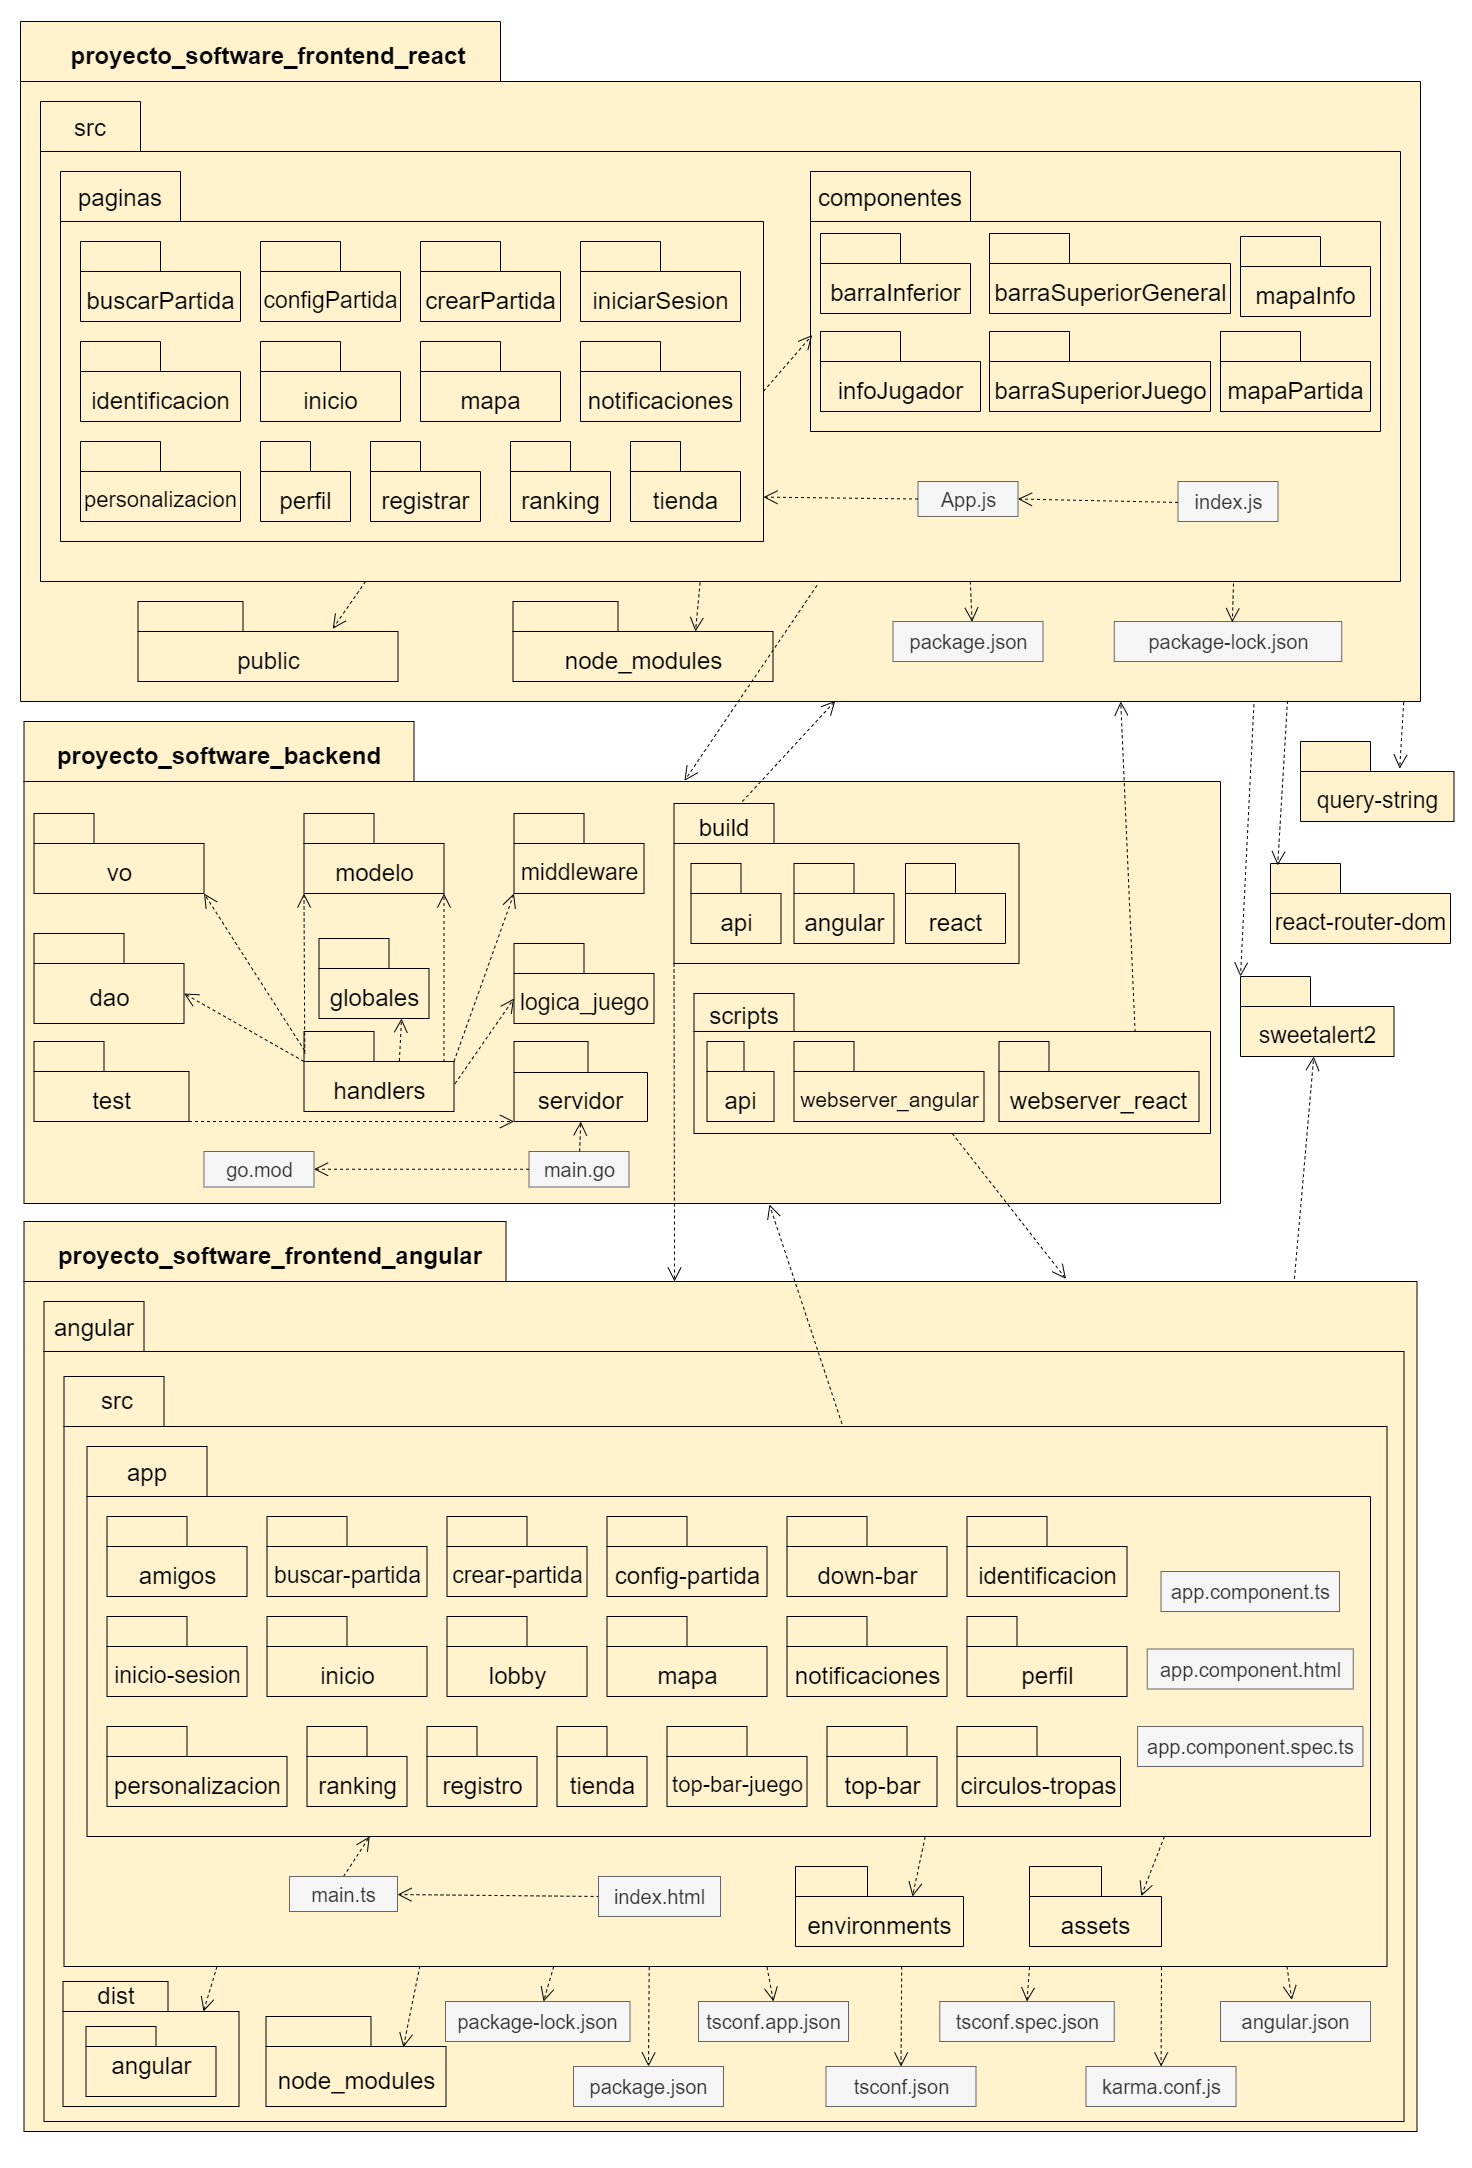
\includegraphics[width=0.9\linewidth]{diagramas/DP.png}
    \caption{Diagrama de paquetes.}
    \label{ref:paquetes}
\end{figure}

\newpage

En siguiente lugar, se ha modelado el \textbf{diagrama de componentes}, apreciable en la Figura \ref{ref:componentes}, en el cual se puede apreciar los dos componentes cliente, uno para cada tecnología. Estos implementan la lógica de presentación y contienen parte de lógica interna de la aplicación, y se comunican con el servidor mediante la misma interfaz (\textit{API}). En siguiente lugar, se encuentra el servidor \textit{web} para la \textit{API}, el cual ofrece una interfaz común a los clientes e implementa la lógica de negocio y el acceso a los datos del sistema. Por último, se encuentra el gestor de base de datos, el cual aporta la persistencia necesaria al sistema. Además, como \textbf{protocolo de comunicación} entre los nodos de la red, se utilizará \textit{HTTP}. \\ \\

\begin{figure}[!h]
    \centering
    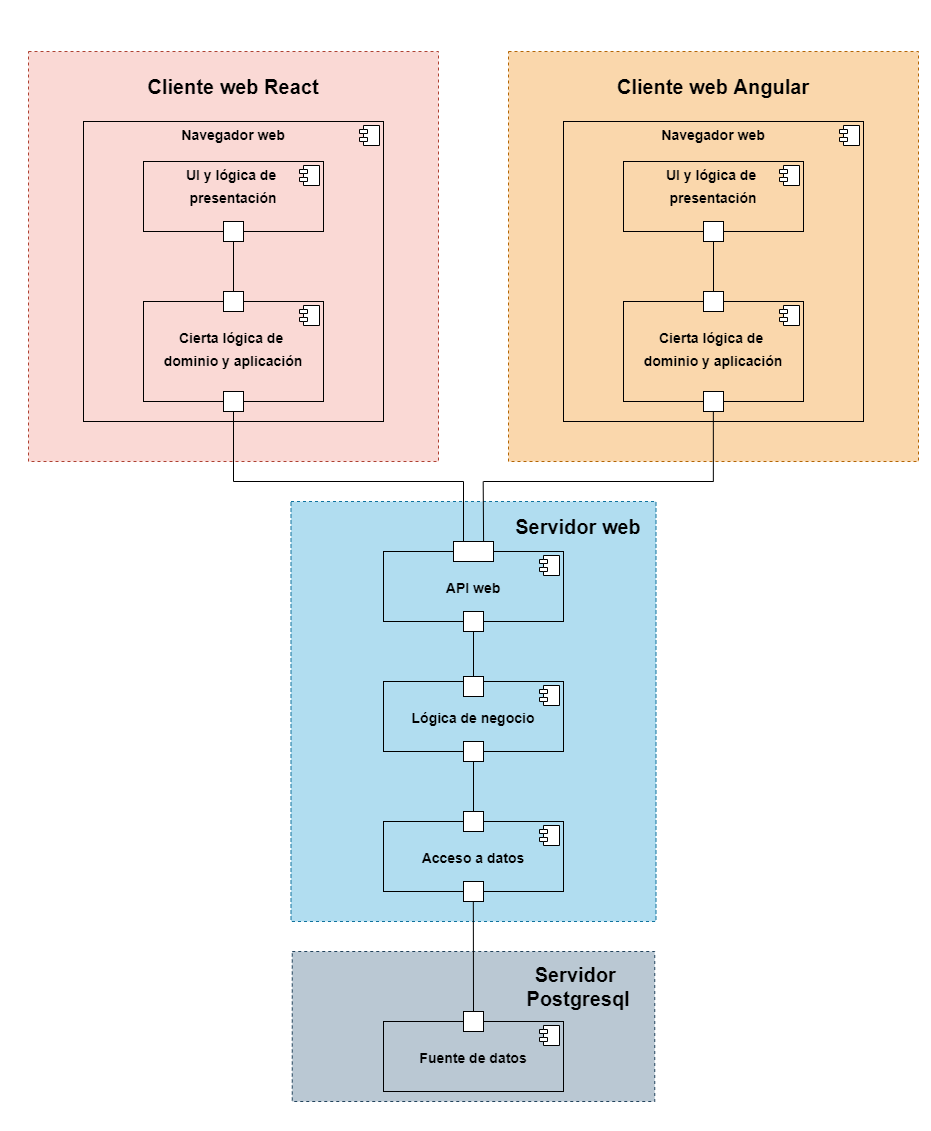
\includegraphics[width=1\linewidth]{diagramas/DC.png}
    \caption{Diagrama de componentes.}
    \label{ref:componentes}
\end{figure}

\newpage

Por otro lado, en la Figura \ref{ref:despliegue} se ilustra el \textbf{diagrama de despliegue}, donde se puede apreciar la distribución de los distintos nodos que componen el sistema. En consecuencia, se ha representado el servidor web de la \textit{API}, contenido en un entorno de ejecución para correspondiente a un contenedor de \textit{Docker}, que ejecuta el código del servidor, y otro entorno con el contenedor para el SGBD \textit{PostgreSQL}. Por otro lado, se encuentran los servidores de React y Angular, cada uno con su entorno de ejecución con un contenedor de \textit{Docker}, que proporcionan el cliente web correspondiente. Por último, se encuentra la máquina del usuario, la cual contiene el entorno de ejecución (navegador web), junto con los artefactos necesarios para ejecutar el cliente correspondiente. \\

\begin{figure}[!h]
    \centering
    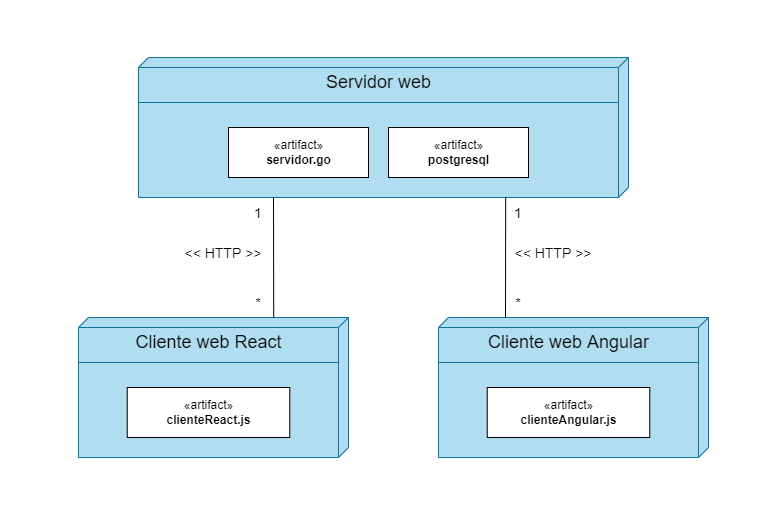
\includegraphics[width=1\linewidth]{diagramas/DD.png}
    \caption{Diagrama de despliegue.}
    \label{ref:despliegue}
\end{figure}

\FloatBarrier

Dadas las características del tipo de aplicación \textit{web}, se va a desarrollar una \textbf{arquitectura cliente-servidor en 3 niveles} como modelo de diseño, en la que los clientes lanzarán peticiones al servidor, este las gestionará y mantendrá el estado del sistema y su persistencia, y devolverá la respuesta correspondiente, que será procesada por la lógica desarrollada en el cliente. \\

\newpage

En la Figura \ref{ref:relacional} aparece el modelo relacional utilizado para la base de datos de la aplicación. Este constará de 5 tablas:
\begin{itemize}
    \item Tabla \textit{Usuario}, en la que se almacenará la información de los distintos usuarios.
    \item Tabla \textit{Partida}, que recogerá la información de las partidas en curso.
    \item Tabla \textit{ItemTienda}, en la que se almacenarán los diferentes elementos de personalización que se podrán comprar a través de la tienda.
    \item Tabla \textit{EsAmigo}, en la que se guardarán las relaciones y solicitudes de amistad entre usuarios.
    \item Tabla \textit{Participa}, en la que se recogerán los usuarios que participan en cada partida.
    \item Tabla \textit{TieneItems}, en la que se almacenarán los elementos de personalización que posee cada usuario.
\end{itemize}
\begin{figure}[!h]
    \centering
    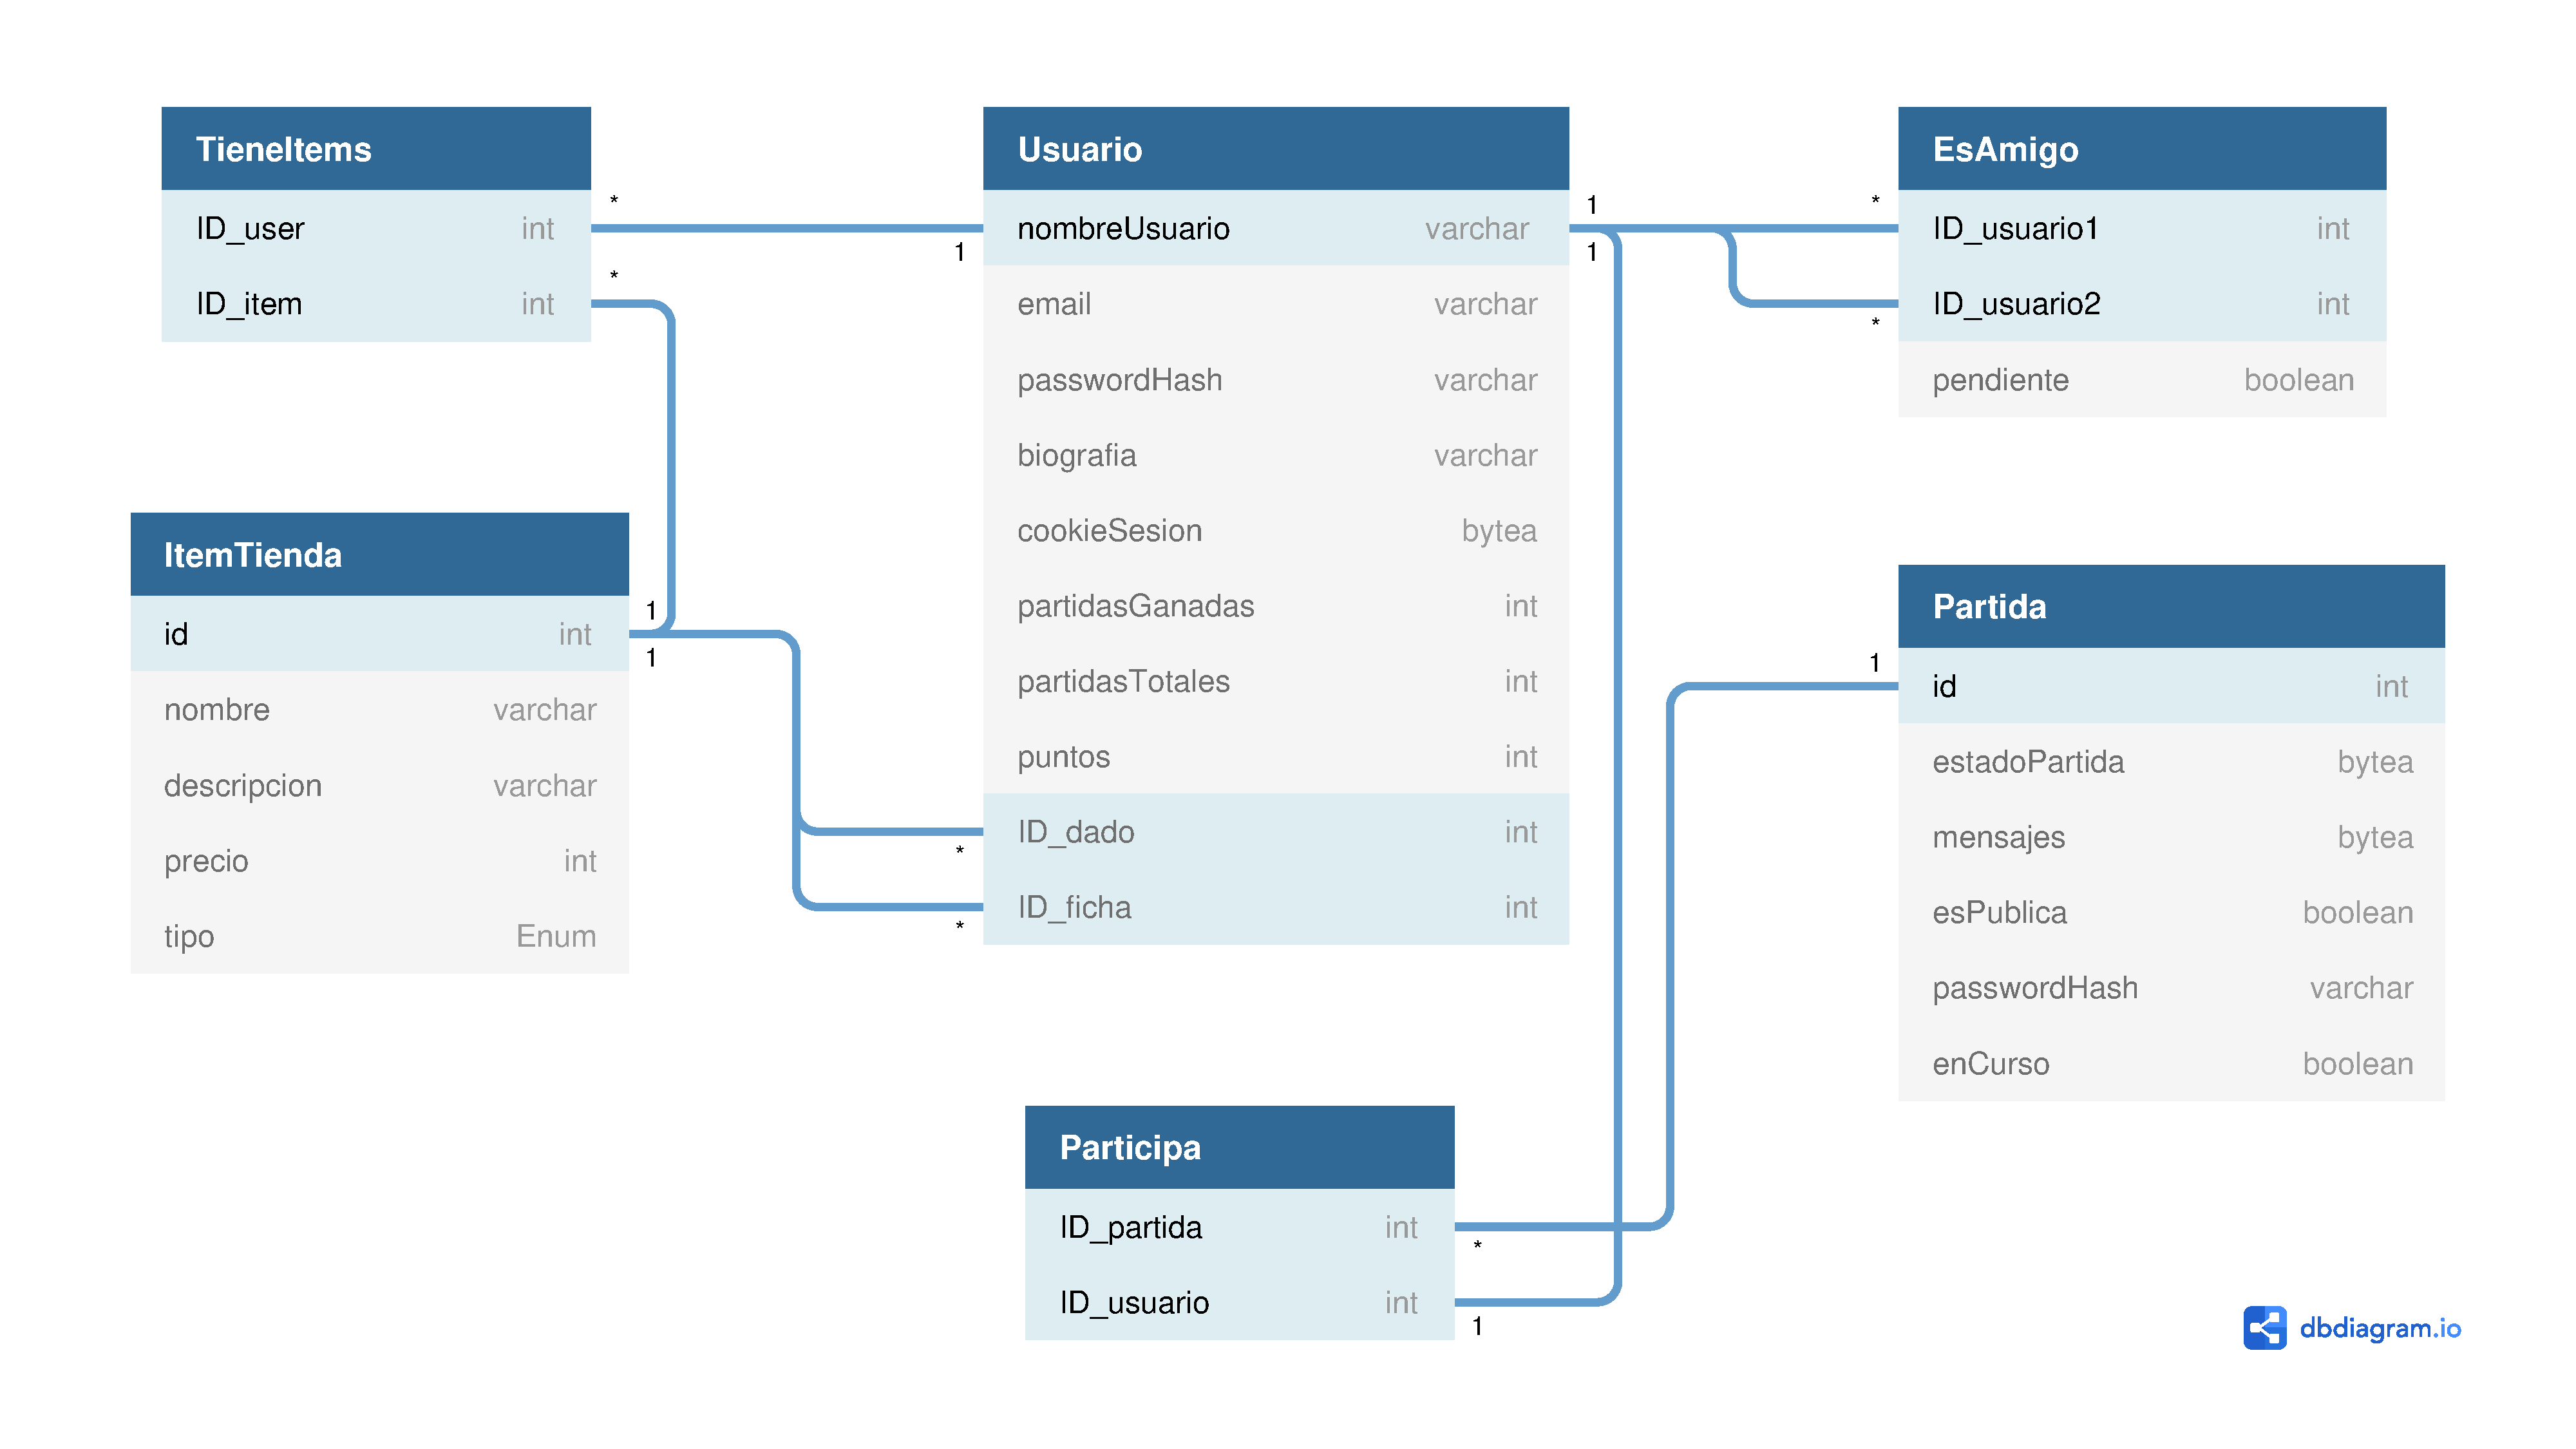
\includegraphics[width=1\linewidth]{diagramas/relacional.pdf}
    \caption{Esquema relacional de la base de datos.}
    \label{ref:relacional}
\end{figure}

Desde el punto de vista de las interfaces del sistema, se ha realizado un diseño completo de la API a consumir por ambos \textit{frontend}. El diagrama de la API, junto a la descripción de los diferentes aspectos implementados, está disponible en el repositorio de documentación\footnote{\href{https://github.com/UNIZAR-30226-2022-01/proyecto_software_documentacion/documentacion_API.md}{\color{blue}{Documentación de la API.}}}. \\

Adicionalmente, todas las funciones públicas del \textit{backend} se han documentado y se encuentran disponibles en la página oficial de documentación de paquetes de Go \footnote{\href{https://pkg.go.dev/github.com/UNIZAR-30226-2022-01/proyecto_software_backend}{\color{blue}{Documentación pública del \textit{backend}.}}}. De esta forma, se permite a ambos equipos de \textit{frontend} acceder a la documentación detallada de cada \textit{endpoint} de la API, que cuenta con ejemplos de respuestas y datos devueltos\footnote{\href{https://pkg.go.dev/github.com/UNIZAR-30226-2022-01/proyecto_software_backend/handlers}{\color{blue}{Documentación de cada \textit{endpoint} del \textit{backend}.}}}.

\subsubsection{Tecnologías elegidas}

En cuanto a las \textbf{tecnologías elegidas}, cabe destacar el uso de \textbf{HTML}, \textbf{CSS} y \textbf{JavaScript} para la parte del frontend de la aplicación, en la que se distinguirá la utilización de dos frameworks de creación de interfaces de usuario: \textbf{React} y \textbf{Angular}. Por ello, la aplicación divergirá en dos clientes ligeramente distintos para el usuario e internamente construidos de distinta forma, que se comunicarán con el servidor web central, el cual no distinguirá entre tipos de clientes, sino que se limitará a atender peticiones, gestionarlas y devolver la respuesta adecuada. \newline

Por otro lado, la tecnología elegida para el servidor o \textbf{backend} es el lenguaje \textbf{Go}, ya que ofrece una gran variedad de herramientas de gestión para un servidor de las características del sistema. Para la persistencia de datos del sistema, se recurrirá al \textit{SGBD} \textbf{PostgreSQL}, ya que cubre con garantías todas las necesidades de la aplicación. \newline

Para el \textit{backend} se ha valorado utilizar las siguientes librerías auxiliares para servir contenidos \textbf{HTTP}:


\begin{itemize}
    \item \textit{Frameworks de web}: Se ha valorado utilizar frameworks web como \textbf{Echo} o \textbf{Gin}. Sin embargo, se ha considerado que  la documentación era escasa en todos los \textit{frameworks} evaluados, y su uso forzaría a una dependencia en las mismas.

    \item Por otro lado, se ha optado por utilizar una librería auxiliar a la librería estándar de \textbf{HTTP} de \textbf{Go}, \textbf{Chi}, que se caracteriza por ser una ampliación a la librería estándar muy sencilla de utilizar, y que permite establecer diferentes \textit{middleware} programables para diferentes \textit{URLs}.

    \item Librerías auxiliares de \textbf{SQL}: Se ha evaluado utilizar \textbf{ORMs} como \textbf{Gorm}, pero se ha considerado que el modelo de datos es lo suficientemente alcanzable como para utilizar la librería \textbf{SQL} y consultas tradicionales.
\end{itemize}

\subsubsection{Aspectos a considerar}

Entre otros \textbf{aspectos a considerar}, cabe destacar los siguientes. El despliegue e instalación de la aplicación se llevará a cabo mediante contenedores de \textbf{Docker}, preferiblemente en un sistema operativo \textbf{Linux}, dada la facilidad de uso y el rápido despliegue que ofrece. Por otro lado, el modelo de datos a implementar se limita al estándar \textbf{SQL}, es decir, un esquema relacional. El servidor ofrece una \textit{API Web} de tipo \textbf{REST}, junto con el uso de \textbf{cookies} para mantener el estado de las sesiones de usuario. \\

Por último, se barajaron otras opciones a las comentadas anteriormente:

\begin{itemize}
    \item Utilizar otro lenguaje para el \textit{backend}, como \textbf{Java}, \textbf{JavaScript} o \textbf{Python}. Sin embargo, se decidió que era más apropiado el uso de \textbf{Go}, ya el equipo está habituado al desarrollo de aplicaciones web con este lenguaje y cubre con garantías las necesidades tecnológicas requeridas.

    \item  Manejar otro sistema gestor de base de datos similar, como un gestor de bases de datos \textbf{NoSQL}. Actualmente existe un amplio abanico de opciones para elegir, y como las necesidades de la aplicación se cubren con prácticamente cualquier gestor, se determinó el uso de \textbf{PostgreSQL}, ya que el equipo está habituado con el uso de este gestor, además de tratarse de uno de los SGBD de código abierto más utilizados y con aspectos muy interesantes.

    \item Existen muchos frameworks para el desarrollo de \textit{frontend web}. Sin embargo, se decidió utilizar  \textbf{React} y \textbf{Angular} porque ofrecen una gran cantidad de recursos que permiten construir interfaces de usuario y toda la lógica asociada a la aplicación. Además, los miembros del equipo mostraban interés para el aprendizaje sobre estas tecnologías tan extendidas en la actualidad.
\end{itemize}

% Entrega 2 y final
\section{Memoria del proyecto}

A continuación se va a describir el inicio y desarrollo del proyecto, desde el punto de vista de cambios realizados respecto a la planificación inicial y de problemas observados durante la implementación del sistema.

\subsection{Inicio del proyecto}
%Apartado react
En relación al equipo del frontend de \textbf{React}, hemos seguido de forma correcta el plan establecido. Hemos seguido los tutoriales correspondientes y, posteriormente, realizamos un proyecto de prueba de cara a probar y poner en práctica las competencias adquiridas. También hemos investigado y probado diversos paquetes o librerías adicionales de \textit{React}, y aprendido a realizar las conexiones con la API y gestionar cookies. Cabe resaltar que \textbf{se han cumplido los objetivos} deseados de acuerdo a la planificación inicial.

% Apartado backend
Con lo que respecta al equipo de \texit{backend}, la formación inicial necesaria no fue tan pesada como en el caso del \texit{frontend}, ya que ambos componentes del equipo tenían experiencia con las tecnologías utilizadas. Aún así ambos consultaron tutoriales y documentación de \textbf{React} y \textbf{Angular} para poder ayudar en el desarrollo del \textit{frontend}, además de los tutoriales sobre diseño de \textit{API} y uso de \LaTeX.

\subsection{Ejecución y control del proyecto}
\subsubsection{Frontend Angular}

El tiempo invertido para la realización de las tareas propuestas no se ha ajustado al plan inicial, y es por ello que no han podido alcanzar los objetivos propuestos en el calendario original. La implementación de algunos aspectos del \textit{frontend} han sido mas costosos de lo esperado, principalmente por la poca del experiencia del equipo al trabajar con el \textit{framework}. La gestión de cookies, y el diseño de una primera versión del mapa fueron las tareas más complejas, y dispararon las horas de trabajo invertidas, escapando del plan inicial.\\

Ambos equipos encargados del \textit{frontend} han aprendido que es muy difícil repartir actividades trabajando en \textit{frameworks} distintos, ya que tratamos de dividir el diseño del mapa entre los 4 integrantes de \textit{frontend}, y a la hora de integrar las tareas realizadas por el equipo de \textit{React} en la implementación de \textit{Angular}, ha sido necesario adaptar el código al \textit{framework}, ya que difieren en multitud de aspectos.

\subsubsection{Frontend React}

%% Repartición de tareas

El trabajo desarrollado por el equipo de \textit{React} ha contado con una muy buena comunicación y coordinación por parte de sus integrantes debido, en gran medida, a haber trabajado juntos en múltiples ocasiones. Esta situación ha propiciado que el entorno de trabajo haya sido cordial y dinámico. \\

La coordinación y el modelo de trabajo han seguido las siguientes indicaciones:

\begin{itemize}
    \item Las decisiones y partes de desarrollo de mayor envergadura o complejidad han sido desarrolladas concurrentemente por los dos integrantes.
    \item Por otro lado, en el resto de ejecuciones se ha optado por realizar dos reuniones semanales de cara a poner en común aspectos realizados, fijar distintos objetivos a lograr o especificar diseños de pantallas.
    \item Por último, se han repartido tareas individuales de forma equitativa, no excesivamente extensas.
\end{itemize}

Como se ha mencionado anteriormente, el \textbf{control de trabajo} de la pareja lo han ido produciendo en las múltiples reuniones realizadas. Por otro lado, se han utilizado los \textit{issues de Git}, de cara a mostrar las tareas realizadas y las pendientes de realizar. \\

Respecto al seguimiento de los procedimientos y herramientas establecidas en un inicio, cabe destacar:

\begin{itemize}
    \item La tecnología elegida inicialmente ha sido adecuada para el desarrollo del sistema, y ha facilitado en gran medida la implementación del mismo debido a la gran cantidad de información y tutoriales que se puede encontrar por la \textit{web} relacionada con \textit{React}.

    \item Cabe destacar que se han añadido o modificado múltiples librerías y paquetes con respecto a los establecidos al inicio del proyecto. Esto se ha debido a que se han ido descubriendo progresivamente ciertos paquetes que, en un principio, no se contaba con utilizar. Los más destacables son:
        \begin{itemize}
            \item \textit{React-router-dom}, de cara a navegar entre las distintas pantallas. \footnote{\href{https://v5.reactrouter.com/web/guides/quick-start}{\color{blue}{\textit{Página oficial react-router-dom.}}}}
            \item \textit{SweetAlert2}, librería de pantallas auxiliares.
            \footnote{\href{https://sweetalert2.github.io}{\color{blue}{\textit{Página oficial SweetAlert2.}}}}
            \item \textit{Query String}, parser de URL.
            \footnote{\href{https://www.npmjs.com/package/query-string}{\color{blue}{\textit{ Página oficial query-string.}}}}
        \end{itemize}
\end{itemize}

Por otro lado, con respecto al \textbf{calendario de tareas} fijado al inicio, no se han cumplido todos los objetivos planeados en un inicio. El motivo reside en que se ha optado por realizar variaciones y priorizar ciertas tareas.
Debido a esto, las pantallas de \textit{Perfil de usuario}, \textit{Búsqueda de partida} y \textit{Buzón de notificaciones} no han sido realizadas para la primera entrega y se ha puesto un mayor enfasis en la implementación del \textit{Mapa de juego}.
Pese a las variaciones comentadas anteriormente, el equipo considera que se han cumplido los objetivos de esta entrega intermedia debido a que la pantalla del \textit{Mapa} se trata de la más compleja de implementar y desarrollar y tiene una importancia relevante sobre todas las demás. \\

Por último, en relación al despliegue del frontend web cabe destacar un problema que surgió, debido a que existen incompatibilidades entre \textit{macOS} y los archivos iniciales de\textit{Docker}. Tras revisar y estudiar el error en prufundidad el equipo consiguió solucionar el problema.

\subsubsection{Backend}

El proceso de ejecución y control del proyecto para el equipo de \textit{backend} se ha considerado satisfactorio.\\

%% Repartición de tareas

En términos de repartición de trabajo, el comienzo del proceso de desarrollo ha consistido en programación en pareja de los aspectos fundamentales del sistema, como la definición del modelo de datos, o la de módulos base, funciones críticas y estructuras a utilizar en el servidor. \\

Una vez realizado esto, se han repartido tareas individuales equitativamente y puesto en común en reuniones más breves todas aquellas funcionalidades comunes a todas las tareas a realizar. \\

%% Tecnologías / librerías elegidas
%% Seguimiento de nombrado de ficheros y formato, etc
%% Seguimiento de control de configuraciones
%% seguimiento de asignación de tareas, issues, etc.
%% control de calidad
%%      tests realizados
%%      control de calidad en commits
%% despliegue

Respecto al seguimiento de los procedimientos establecidos, se han seguido los siguientes aspectos con éxito:

\begin{itemize}
    \item Las tecnologías y librerías elegidas inicialmente han sido adecuadas para el desarrollo del sistema, y han facilitado en gran medida la implementación del mismo, gracias a la libería estándar de \textit{Go} y el framework \textit{Chi}.

    \item El seguimiento de las reglas de formato y documentación de código se han seguido fácilmente debido a las herramientas proporcionadas por \textit{Go}, como \textit{godoc} o \textit{gofmt}.

    \item Se ha realizado un seguimiento y asignación de las tareas a realizar mediante incidencias de \textit{Github},  listas de tareas en cada uno de ellos e hitos, tal y como se había acordado.

    \item Se han realizado test automáticos para cada funcionalidad base implementada, que corresponde a un conjunto de llamadas a la \textit{API} relacionadas con un mismo aspecto del sistema, como la gestión de amigos o la implementación de una fase del juego.

    Así mismo, se ha conseguido fácilmente que dichos test se comporten como un cliente del sistema gracias a la librería estándar de \textit{Go}.

    \item Se ha vigilado en todo momento que los commits fueran correctos tal y como ha sido establecido, y que se completaran los test automáticos con éxito antes de subirlos.

    \item Se ha conseguido automatizar un despliegue completo de cada uno de los \textit{frontend} y del servidor de la \textit{API} para facilitar las pruebas exploratorias y de comportamiento del sistema fuera de los test automáticos.
\end{itemize}

% discutir como se ha seguido el calendario

Por otro lado, se ha conseguido seguir el calendario de tareas establecido en todo momento, llegando a implementar una versión inicial del juego, consistente en el inicio y la gestión de las partidas y la primera fase de un turno, así como todos los aspectos fundamentales del diseño del sistema (el modelo de datos, autenticación de usuarios o una versión preliminar de toda la \textit{API}, por ejemplo) y funcionalidades adicionales como los aspectos sociales del juego.\\

La única divergencia respecto a la planificación inicial ha sido el aplazamiento de la implementación de la \textit{API} de notificaciones una semana, aún dentro del límite, debido a que se ha detectado que dependía de funcionalidades de la lógica de juego. \\

\newpage

Por último, durante el desarrollo del sistema se han detectado los siguientes problemas respecto al control de versiones, construcción y despliegue del software:
\begin{itemize}
    \item Al realizar pruebas exploratorias de los \textit{frontend} con el despliegue automático de contenedores de \texit{Docker}, se han experimentado problemas no observados al realizar los test automáticos debido a que los servidores de \textit{frontend} y \textit{backend} se encontraban en dominios diferentes.

    Esto ha requerido realizar cortas reuniones con ambos equipos e implementar un middleware de \textit{CORS} \footnote{\href{https://developer.mozilla.org/en-US/docs/Web/HTTP/CORS}{\color{blue}{\textit{ Información sobre CORS por Mozilla.}}}}. Adicionalmente, esto ha provocado problemas inesperados con el tratamiento de \textit{cookies} que también ha requerido reuniones con ambos equipos.

    \item El despliegue automático ha requerido ligeros cambios para que fuera posible su ejecución en equipos con \textit{macOS}.
\end{itemize}

\subsection{Control del rendimiento}
Para comprobar el correcto rendimiento de los miembros del equipo, así como la evolución del mismo a lo largo del desarrollo, se han recogido y evaluado diferentes métricas de \texit{Github} al final del mismo. Esto ha sido posible gracias a que se ha hecho uso de \textit{issues} e hitos para realizar el control de tareas, y a que \textit{Github} recoge métricas de \textit{commits} realizados y sus cambios.

\subsubsection{Control de incidencias e hitos} % Renombrar, lo que se me ha ocurrido

\subsubsection{Control de \textit{commits} realizados}
Una medida útil para comprobar el trabajo realizado por cada uno de los miembros del equipo a lo largo del tiempo es el análisis de los \textit{commits} realizados. Estos permiten identificar los periodos de mayor actividad para cada miembro, así como una visión muy general del trabajo realizado. 

Cabe mencionar que los \textit{commits} realizados por un miembro no son representativos de su carga de trabajo. Esto se puede apreciar en los equipos de ambos \textit{frontend}, donde debido a la naturaleza de las tareas (implementaciones de pantallas, ya sean complejas o simples) hay números dispares de \textit{commits} entre unos miembros y otros, y una cantidad menor respecto al equipo de \textit{backend}.

\begin{figure}[!h]
    \centering
    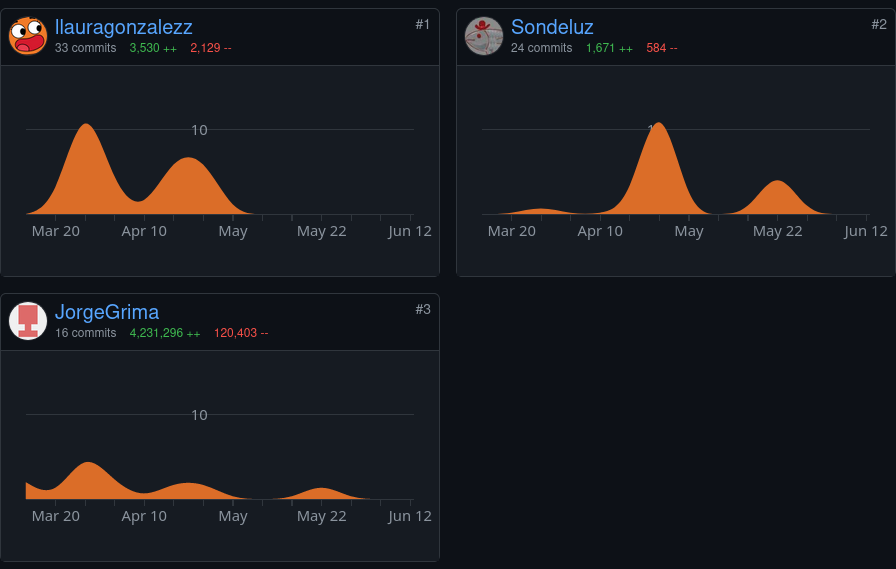
\includegraphics[scale=0.35]{metricas/commits_angular.png}
    \caption{\textit{Commits} realizados en el repositorio de \textit{Angular}. Cabe mencionar que, por razones desconocidas, \textit{Github} no muestra los commits realizados por Laura durante las últimas semanas. Así mismo, se puede observar la incorporación de Samuel al terminar las funcionalidades principales del \textit{Backend}.}
    \label{fig:my_label}
\end{figure}

\begin{figure}[!h]
    \centering
    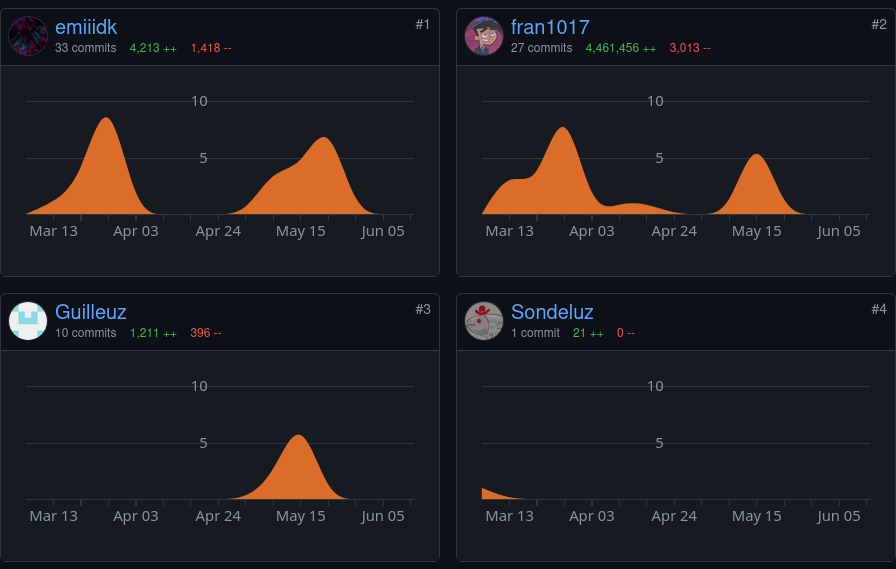
\includegraphics[scale=0.35]{metricas/commits_react.png}
    \caption{\textit{Commits} realizados en el repositorio de \textit{React}. Del mismo modo que en el repositorio de \textit{Angular}, se puede observar la incorporación de Guillermo al terminar las funcionalidades principales del \textit{Backend}.}
    \label{fig:my_label}
\end{figure}

\begin{figure}[!h]
    \centering
    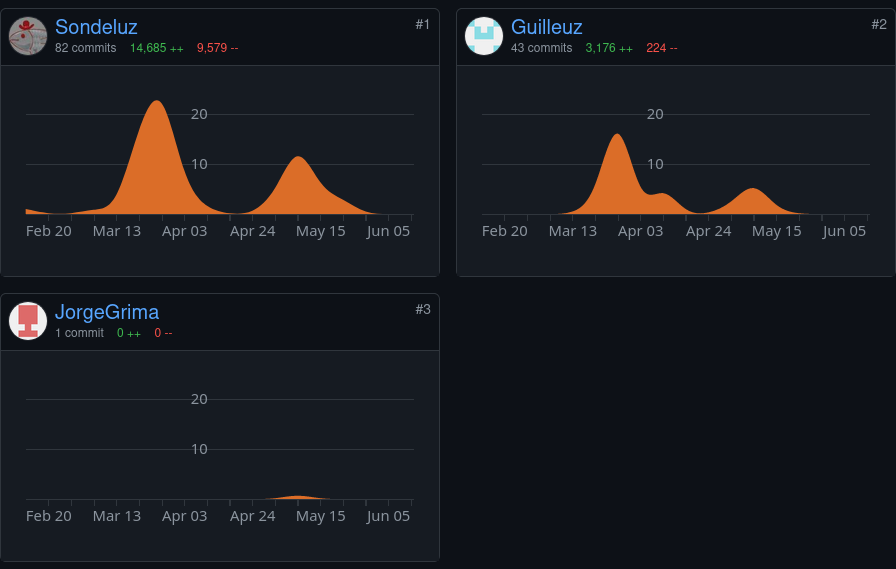
\includegraphics[scale=0.35]{metricas/commits_backend.png}
    \caption{\textit{Commits} realizados en el repositorio de \textit{Backend}.}
    \label{fig:my_label}
\end{figure}
\FloatBarrier
En todos los casos se puede observar como los periodos de actividad de cada miembro han sido similares, y coinciden con los momentos en los que había un mayor número de tareas planificadas, así como con la cercanía de las entregas intermedia y la final.

Adicionalmente, se puede observar que la mayor actividad ha ocurrido durante la fase inicial del proyecto, que corresponde a implementar los módulos, pantallas y funcionalidades principales. Así mismo, es notable la reducción de la actividad en el \textit{backend} al final del proyecto, que corresponde con la finalización de las funcionalidades principales y la incorporación de cada uno de los miembros a los \textit{frontend}.\\

Por otro lado, los cambios realizados por los \textit{commits} permiten observar los cambios realizados en cada una de las partes del proyecto a lo largo del tiempo. Estos cambios están medidos en líneas añadidas y borradas como \textit{Code Churn}, donde una gran cantidad de cambios en fases finales del proyecto puede indicar un mal planteamiento o seguimiento de las tareas del mismo. 

Para evaluar esto se ha utilizado como referencia el \textit{backend}, debido a que se ha tenido que refactorizar el código múltiples veces, al subestimar el tamaño y complejidad de la implementación de algunos módulos.

\begin{figure}[!h]
    \centering
    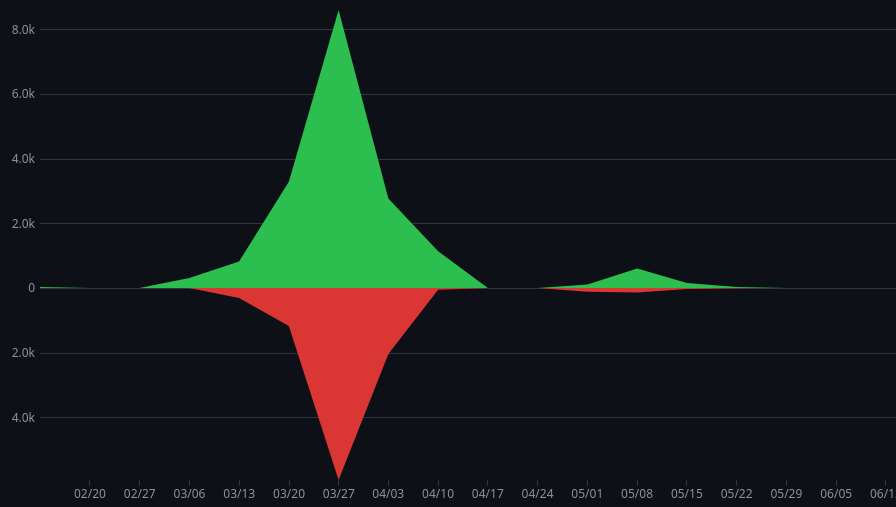
\includegraphics[scale=0.35]{metricas/code_churn_backend.png}
    \caption{\textit{Code Churn} del backend.}
    \label{fig:my_label}
\end{figure}
\FloatBarrier

Se puede observar como el mayor número de cambios ha ocurrido durante el inicio y la entrega intermedia del proyecto, coincidiendo con las refactorizaciones. Así mismo, es fácil observar que se han modificado y añadido funcionalidades de pequeño tamaño durante la fase final, que coincide con la recepción del \textit{feedback} de la API del juego por parte de los equipos de \textit{frontend}.

\subsection{Cierre del proyecto}

El proyecto, al dividirse en tres partes bien diferenciadas, cuenta con tres ritmos de trabajo distintos. Pese a eso, hemos conseguido en gran medida una gran compenetración entre todos los equipos y hemos logrado en gran medida, hasta la fecha, los objetivos iniciales establecidos. A continuación, se pondrá énfasis en el análisis de los resultados obtenidos frente a las estimaciones iniciales. \\

\subsubsection{Cierre del proyecto por el equipo de \textit{Backend}}
El tiempo utilizado para la realización de las distintas tareas del \textbf{Backend} se ajusta razonablemente a la estimación inicial.
Aún así, a la hora de realizar el proyecto hemos podido comprobar que las tareas elegidas para las estimaciones eran demasiado generales.\\

Principalmente, englobar la lógica del juego como una sola tarea ha dificultado una estimación temporal más precisa. En la práctica, dicha tarea fue dividida en distintas partes, principalmente enel diseño de la máquina de estados, la implementación del mapa y la de las diferentes fases de juego. Creemos que estas divisiones se podrían haber realizado al inicio del proyecto, analizando más exhaustivamente el funcionamiento del juego para permitir estimaciones más precisas. \\

Mencionamos también que, aunque no se hubiera tenido en cuenta en la estimación inicial, el tiempo empleado en la implementación de las pruebas fue muy elevado, y habría sido conveniente haberlo tenido en cuenta durante la planificación de tareas. \\

Destacamos que si el desarrollo del \textit{backend} sigue progresando al ritmo actual, se acabará su implementación antes de lo planeado en el calendario. De esta forma, los encargados del \textit{backend} podrán ayudar en la implementación de los \textit{frontend}, encargándose además de modificar y corregir el backend cuando sea necesario. \\

Una de las principales lecciones que hemos aprendido durante el desarrollo del \textit{backend}, es que debemos gestionar y modularizar el código, no solo en distintos componentes, si no en diferentes ficheros de código. Debido a esto, se han tenido que dedicar múltiples reuniones, aunque de corta duración, a la refactorización del código.\\

Adicionalmente, la magnitud del proyecto ha fomentado a realizar \textit{commits} más concisos y frecuentes. \\

\subsubsection{Cierre del proyecto por el equipo de \textit{React}}
Por otro lado, desde el punto de vista del frontend desarrollado en \textbf{React}, pese a haber subestimado esfuerzos que se tenían que dedicar en ciertas partes del sistema, como puede ser el mapa, hemos conseguido mantener y conseguir mayoritariamente los objetivos iniciales. Además, creemos que se conseguirán conseguir los objetivos finales en el plazo establecido. \\

Cabe destacar que las pequeñas divergencias entre las estimaciones iniciales y el coste y esfuerzos reales se deben, en gran medida, a la falta de experiencia en la realización de proyectos de tal envergadura. Es por eso, que se quiere recalcar la experiencia que hemos adquirido de cara a establecer estimaciones iniciales con mayor eficacia en futuros proyectos. \\


\subsubsection{Cierre del proyecto por el equipo de \textit{Angular}}

El tiempo invertido para la realización de las tareas propuestas no se ha ajustado al plan inicial, y es por ello que no han podido alcanzar los objetivos propuestos en el calendario original. La implementación de algunos aspectos del \textit{frontend} han sido mas costosos de lo esperado, principalmente por la poca del experiencia del equipo al trabajar con el \textit{framework}. La gestión de cookies, y el diseño de una primera versión del mapa fueron las tareas más complejas, y dispararon las horas de trabajo invertidas, escapando del plan inicial.
\\

Ambos equipos encargados del \textit{frontend} han aprendido que es difícil repartir actividades trabajando en \textit{frameworks} distintos, ya que tratamos de dividir el diseño del mapa entre los 4 integrantes de \textit{frontend}, y a la hora de integrar las tareas realizadas por el equipo de \textit{React} en la implementación de \textit{Angular}, ha sido necesario adaptar el código al \textit{framework}. \\


\subsubsection{Valoraciones comunes entre todos los equipos}

Durante el desarrollo del \textit{backend}, hemos podido aprender sobre el \textit{CORS} y las peticiones de datos de origen cruzado, al servir los clientes web y la API desde dominios diferentes. Así mismo, hemos ganado experiencia en el despliegue y depuración de contenedores con \textit{Docker}. \\

Así mismo, durante el desarrollo de los \textit{frontend}, cabe destacar el avance y aprendizaje obtenido en el desarrollo y creación de interfaces, \textit{UX design}.\\

% Esfuerzos realizados
Los esfuerzos realizados por los integrantes del equipo han sido los siguientes:

\begin{itemize}
    \item En primer lugar, \textbf{Guillermo} invirtió un total de 34 horas, encargándose de implementar la fase de refuerzo, las funciones de creación y configuración de partidas, la implementación de la baraja y otras funciones sociales.

    \item \textbf{Samuel} se encargó de desarrollar la fase inicial del juego, la gestión de las listas de amigos, la configuración del \textit{CORS}, el despliegue de la aplicación y su automatización, la generación automática de documentación con la herramienta \textit{godoc}, el sistema de búsqueda de partidas y las notificaciones.
    
    Durante la entrega final, se encargó de la fase final del juego, el despliegue automático en la nube, el uso de \textit{TLS}, el reseteo de contraseñas, el envío de coreos electrónicos, la gestión de partidas terminadas y expulsiones de jugadores y las notificaciones. Así mismo, pasó a ayudar al equipo de \textit{Angular} en el desarrollo del autómata del juego y las pantallas de tienda y personalización, entre otras tareas.
    
    En total, invirtió 147 horas.

    \item \textbf{Fran} desarrolló junto con el resto del grupo de \textit{frontend} el diseño del mapa de juego. Además, la implementación de diversas pantallas como \textit{Registro Usuario, Inicio Sesión y Crear Partida}, entre otras. También, realizó dinámica adicional del mapa como ciertos botones, un mapa informativo o pantallas de avisos. En conjunto dedicó un estimado de 37 horas.

    \item \textbf{Emilio} dedicó un total de 41 horas a las tareas asignadas, entre las que destacan la puesta en marcha inicial del cliente, conexiones con la API y su gestión de errores, mantenimiento de cookies, implementación y diseño de pantallas y elementos gráficos, y redacción, maquetación y diseño de apartados de la memoria.

    \item \textbf{Jorge} diseñó de las pantallas de inicio de sesión y registro de usuario. También realizó el diseño del mapa, tratando de aprender cuestiones básicas sobre \textit{svg}, transiciones en angular, y otros elementos de diseño que proporciona la herramienta. Además, realizó la pantalla de búsqueda de partida, en la cual fue necesario aprender nuevos aspectos de diseño y cuestiones básicas sobre conexiones a la API. En total, invirtió 32 horas.

    \item \textbf{Laura} realizó el diseño de las pantallas de inicio de sesión y registro de usuario, también se encargó de realizar la conexión de las pantallas de inicio de sesión y registro la API. Además, implementó el diseño diseño y conexión con la API para la pantalla de crear partida. También, realizó el diseño y la funcionalidad de las 2 \textit{top-bar} y la \textit{bottom-bar} que usarán ambos \textit{frontend}. En conjunto dedicó un estimado de 36 horas.
    %% Continuar aqui el resto
\end{itemize}

\section{Conclusiones}
Unificar todas

\subsection{React}
\subsection{Angular}
\subsection{Backend}
\begin{itemize}
    \item Realizar una planificación de la organización en módulos del código a desarrollar en mayor detalle, así como del conjunto de \textit{endpoints} de API a exponer. Hemos tenido que realizar múltiples \textit{refactoring} del código para acomodar nuevas funcionalidades. Así mismo, se han tenido que establecer nuevos \textit{endpoints} y modificar los existentes una vez los \textit{frontend} han empezado a consumirlos.
    
    Aunque entendemos que esto es algo que mejora con la experiencia, este aspecto nos ha afectado especialmente, puesto que se había infravalorado su importancia al empezar el desarrollo del proyecto.
    
    \item El despliegue en un entorno real de la aplicación se haría en una etapa más temprana. Aunque no han ocurrido problemas significativos durante el mismo en este proyecto, podría haber sido posible que fueran necesarios cambios significativos en el código y las tecnologías utilizadas para trabajar con proveedores externos para funcionalidades como, por ejemplo, el envío de correo electrónico.
    
    Realizar un despliegue real preliminar durante las primeras etapas del desarrollo, aunque sea incompleto, sería beneficioso para identificar posibles errores y cambios necesarios.
\end{itemize}

\subsection{Generales}
\begin{itemize}
    \item Se intentaría explorar herramientas que apoyen la definición y repartición de tareas entre los diferentes equipos y sus miembros. Aunque hemos hecho uso de \textit{issues} e hitos de \textit{Github} para ello, consideramos que la funcionalidad que ofrece es demasiado básica. Por ello, proyectos más complejos se podría explorar el uso de herramientas como Trello\footnote{\href{https://trello.com/es}{\color{blue}{\textit{Trello.}}}}.
\end{itemize}
%\clearpage
%\section{Anexos}
%\subsection{Glosario}
%\subsection{Actas de todas las reuniones realizadas}

%\newpage
%\section{Referencias}
%\subsection{Bibliografía}
%\printbibliography

%\newpage
%\section{Anexos}
%\subsection{Diagrama de la API del sistema}
%\label{anexo:A}
%\markdownInput{diagramas/API.md}

\end{document}
